% \begin{name}
% 	{GV biên soạn: Nguyễn Tuấn\\ GV phản biện 1: Nhất Linh}
% 	{TOÁN 10-KNTT-CS}
% \end{name}
%----------------NỘI DUNG BIÊN SOẠN
\setcounter{section}{21}
\section{Ba đường cônic}
%-------------------------------------------
\subsection{KIẾN THỨC TRỌNG TÂM}
\subsubsection{Elip}
\begin{dn}
\immini{
	Cho hai điểm cố định $F_1$, $F_2$ và độ dài $F_1F_2=2c>0$.\\
	\textbf{Đường elip $(E)$} hay elip $(E)$ là tập hợp các điểm $M$ trong mặt phẳng sao cho $MF_1+MF_2=2a$, với $a$ là số thực dương cho trước và $a>c$.\\
	Ta viết gọn như sau
	$$(E)= \{M\mid MF_1+MF_2=2a\,,\text{với } a>c\}.$$
	Hai điểm $F_1$ và $F_2$ gọi là hai \textbf{tiêu điểm} của elip $(E)$.\\
	Độ dài $F_1F_2=2c$ gọi là \textbf{tiêu cự} của elip.
}{
	\begin{tikzpicture}[scale=0.6, font=\footnotesize, line join=round, line cap=round, >=stealth]
		\def\a{2.4};
		\def\b{1.6};
		\pgfmathsetmacro\c{sqrt((\a)^2-(\b)^2)};
		\draw[name path=e] (0,0) ellipse (\a cm and \b cm);
		\path
		($(0,0) + (60:{\a} and {\b})$) coordinate (M)
		(-\c,0) coordinate (F_1)
		(\c,0) coordinate (F_2)
		($(M)+(108:0.4)$) coordinate (A)
		($(M)+(140:0.4)$) coordinate (B)
		($(A)+(124:2)$) coordinate (D)
		($(B)+(D)-(A)$) coordinate (C)
		($(C)!0.5!(D)$) coordinate (E)
		;
		\foreach \i/\j in {M/above right,F_1/below,F_2/below}
		\draw[fill=black] (\i) circle(1pt) node[\j]{$\i$};
		\draw (M)--(F_1)--(F_2)--(M);
		%cây viết
		\draw (A)--(M)--(B);
		\fill[gray,draw=black] (A)--(B)--(C)--(D)--(A);
		\fill[rotate=34,white,draw=black] (D) arc(0:360:0.11 and 0.05);
		\fill[rotate=34,black] (E) ellipse (0.05 and 0.025);
	\end{tikzpicture}
}
\end{dn}
\begin{tc}
	\immini{
	Chọn hệ trục toạ độ $Oxy$ như hình vẽ bên. Khi đó phương trình chính tắc của  đường elip $(E)$ có dạng là
	$$\dfrac{x^2}{a^2}+\dfrac{y^2}{b^2}=1\,,\heva{&a>b>0\\
		&c^2=a^2-b^2.}$$
}{
	\begin{tikzpicture}[scale=0.6, font=\footnotesize, line join=round, line cap=round, >=stealth]
		\def\a{2.4};
		\def\b{1.6};
		\pgfmathsetmacro\c{sqrt((\a)^2-(\b)^2)};
		\draw[->] ($(-{\a},0)-(1,0)$)--($({\a},0)+(1,0)$) node[above]{$x$};
		\draw[->] ($(0,-{\b})-(0,1)$)--($(0,{\b})+(0,1)$) node[left]{$y$};
		\draw[name path=e] (0,0) ellipse (\a cm and \b cm);
		\path
		(0,0) coordinate (O)
		($(0,0) + (55:{\a} and {\b})$) coordinate (M)
		(-\c,0) coordinate (F_1)
		(\c,0) coordinate (F_2)
		(-\a,0) coordinate (A_1)
		(\a,0) coordinate (A_2)
		(0,-\b) coordinate (B_1)
		(0,\b) coordinate (B_2)
		;
		\foreach \i/\j in {F_1/below,F_2/below,O/below left,A_1/below left,A_2/below right,B_1/below right,B_2/above right}
		\draw[fill=black] (\i) circle(1pt) node[\j]{$\i$};
		\draw[fill=black] (M) circle(1pt) node[above right]{$M(x;y)$};
		\draw (M)--(F_1) (F_2)--(M);
	\end{tikzpicture}
}
\end{tc}
\begin{nx}
	{\bf Các yếu tố của elip}\\
		Cho elip $(E)$ có phương trình chính tắc là $$\dfrac{x^2}{a^2}+\dfrac{y^2}{b^2}=1\,,\heva{&a>b>0\\
		&c^2=a^2-b^2.}$$
	Khi đó:
	\begin{itemize}
		\item $(E)$ cắt $Ox$ tại hai điểm $A_1(-a;0)$, $A_2(a;0)$ và cắt $Oy$ tại hai điểm $B_1(0;-b)$, $B_2(0;b)$ và các điểm $A_1$, $A_2$, $B_1$, $B_2$ được gọi là các \textbf{đỉnh} của elip.
		\item Đoạn thẳng $A_1A_2=2a$ gọi là \textbf{ độ dài trục lớn}, đoạn thẳng $B_1B_2=2b$ gọi là \textbf{ độ dài trục nhỏ} của elip.
		\item Hai \textbf{tiêu điểm} của elip là $F_1(-c;0)$ và $F_2(c;0)$.
		\item Độ dài $F_1F_2=2c$ gọi là \textbf{tiêu cự} của elip.
		\item Với điểm $M(x;y)\in (E)$ thì $\dfrac{x^2}{a^2}+\dfrac{y^2}{b^2}=1$ và $|x|\le a$, $|y|\le b$.
		\item Giao điểm $O$ của hai trục gọi là \textbf{tâm đối xứng} của elip.
		\item Hai trục $Ox$, $Oy$ là hai \textbf{trục đối xứng} của elip.
	\end{itemize}
\end{nx}
\subsubsection{Hypebol}
\begin{dn}
	\immini{
	Cho hai điểm cố định $F_1$, $F_2$ và độ dài $F_1F_2=2c>0$.\\
	\textbf{Đường hypebol $(H)$} hay hypebol $(H)$ là tập hợp các điểm $M$ trong mặt phẳng sao cho $\left|MF_1-MF_2\right|=2a$, với $a$ là số thực dương cho trước và $a<c$.\\
	Ta viết gọn như sau
	$$(H)= \{M\mid \left|MF_1-MF_2\right|=2a\,,\text{với } a<c\}.$$
	Hai điểm $F_1$ và $F_2$ gọi là hai \textbf{tiêu điểm} của hypebol $(H)$.\\
	Độ dài $F_1F_2=2c$ gọi là \textbf{tiêu cự} của hypebol.
}{
	\begin{tikzpicture}[scale=0.7, font=\footnotesize, line join=round, line cap=round, >=stealth]
		\def\a{1.2};
		\def\b{1};
		\pgfmathsetmacro\c{sqrt((\a)^2+(\b)^2)};
		\draw[name path=h1,smooth, samples=200, domain=\a:2.5] plot (\x,{((\b)/(\a))*sqrt((\x)^2-(\a)^2)});
		\draw[yscale=-1,name path=h2,smooth, samples=200, domain=\a:2.5] plot (\x,{((\b)/(\a))*sqrt((\x)^2-(\a)^2)});
		\draw[xscale=-1,name path=h2,smooth, samples=200, domain=\a:2.5] plot (\x,{((\b)/(\a))*sqrt((\x)^2-(\a)^2)});
		\draw[xscale=-1,yscale=-1,name path=h2,smooth, samples=200, domain=\a:2.5] plot (\x,{((\b)/(\a))*sqrt((\x)^2-(\a)^2)});
		\def\xm{2};
		\pgfmathsetmacro\ym{((\b)/(\a))*sqrt((\xm)^2-(\a)^2)};
		\path
		(0,0) coordinate (O)
		(-\c,0) coordinate (F_1)
		(\c,0) coordinate (F_2)
		(-\a,0) coordinate (A_1)
		(\a,0) coordinate (A_2)
		(\xm,\ym) coordinate (M)
		;
		\draw[fill=black] (F_1) circle(1pt) node[below]{$F_1$};
		\draw[fill=black] (F_2) circle(1pt) node[below]{$F_2$};
		\draw[fill=black] (M) circle(1pt) node[right]{$M(x;y)$};
		\draw (F_1)--(M)--(F_2)--(F_1);
	\end{tikzpicture}
}
\end{dn}
\begin{tc}
	\immini{
	Chọn hệ trục toạ độ $Oxy$ như hình vẽ bên. Khi đó phương trình chính tắc của  đường hypebol $(H)$ có dạng là
	$$\dfrac{x^2}{a^2}-\dfrac{y^2}{b^2}=1\,,\heva{&a,b>0\\
		&c^2=a^2+b^2.}$$
}{
	\begin{tikzpicture}[scale=0.7, font=\footnotesize, line join=round, line cap=round, >=stealth]
		\def\a{1.2};
		\def\b{1};
		\pgfmathsetmacro\c{sqrt((\a)^2+(\b)^2)};
		\draw[->] ($(-{\a},0)-(1.5,0)$)--($({\a},0)+(1.5,0)$) node[above]{$x$};
		\draw[->] ($(0,-{\b})-(0,1)$)--($(0,{\b})+(0,1)$) node[left]{$y$};
		\draw[name path=h1,smooth, samples=200, domain=\a:2.5] plot (\x,{((\b)/(\a))*sqrt((\x)^2-(\a)^2)});
		\draw[yscale=-1,name path=h2,smooth, samples=200, domain=\a:2.5] plot (\x,{((\b)/(\a))*sqrt((\x)^2-(\a)^2)});
		\draw[xscale=-1,name path=h2,smooth, samples=200, domain=\a:2.5] plot (\x,{((\b)/(\a))*sqrt((\x)^2-(\a)^2)});
		\draw[xscale=-1,yscale=-1,name path=h2,smooth, samples=200, domain=\a:2.5] plot (\x,{((\b)/(\a))*sqrt((\x)^2-(\a)^2)});
		\def\xm{2};
		\pgfmathsetmacro\ym{((\b)/(\a))*sqrt((\xm)^2-(\a)^2)};
		\path
		(0,0) coordinate (O)
		(-\c,0) coordinate (F_1)
		(\c,0) coordinate (F_2)
		(-\a,0) coordinate (A_1)
		(\a,0) coordinate (A_2)
		(\xm,\ym) coordinate (M)
		;
		\draw[fill=black] (O) circle(1pt) node[below left]{$O$};
		\draw[fill=black] (F_1) circle(1pt) node[below]{$F_1$};
		\draw[fill=black] (F_2) circle(1pt) node[below]{$F_2$};
		\draw[fill=black] (M) circle(1pt) node[right]{$M(x;y)$};
		\draw (F_1)--(M)--(F_2);
	\end{tikzpicture}
}
\end{tc}
\begin{nx}
{\bf Các yếu tố của hypebol}\\
	Cho hypebol $(H)$ có phương trình chính tắc là $$\dfrac{x^2}{a^2}-\dfrac{y^2}{b^2}=1\,,\heva{&a,b>0\\
	&c^2=a^2+b^2.}$$
Khi đó:
\begin{itemize}
	\item $(E)$ cắt $Ox$ tại hai điểm $A_1(-a;0)$, $A_2(a;0)$ và các điểm $A_1$, $A_2$ được gọi là các \textbf{đỉnh} của hypebol.
	\item Đoạn thẳng $A_1A_2=2a$ gọi là \textbf{ độ dài trục thực}, đoạn thẳng $B_1B_2=2b$ gọi là \textbf{ độ dài trục ảo} của hypebol.
	\item Hai \textbf{tiêu điểm} của hypebol là $F_1(-c;0)$ và $F_2(c;0)$.
	\item Độ dài $F_1F_2=2c$ gọi là \textbf{tiêu cự} của hypebol.
	\item Với điểm $M(x;y)\in (H)$ thì $\dfrac{x^2}{a^2}-\dfrac{y^2}{b^2}=1$ và $x\le -a$ hoặc $x\ge a$.
	\item Giao điểm $O$ của hai trục gọi là \textbf{tâm đối xứng} của hypebol.
	\item Hai trục $Ox$, $Oy$ là hai \textbf{trục đối xứng} của hypebol.
\end{itemize}
\end{nx}
\subsubsection{Parabol}
\begin{dn}
	\immini{
	Cho một điểm $F$ và một đường thẳng $\Delta$ cố định không đi qua $F$. Parabol $(P)$ là tập hợp các điểm $M$ cách đều $F$ và $\Delta$.\\
	$F$ gọi là \textbf{tiêu điểm} và $\Delta$ gọi là \textbf{đường chuẩn} của parabol $(P)$.
}{
	\begin{tikzpicture}[scale=0.8, font=\footnotesize, line join=round, line cap=round, >=stealth]
		\def\xm{-1.3};
		\pgfmathsetmacro\ym{0.5*(\xm)^2};
		\path
		(0,0) coordinate (O)
		(0,0.5) coordinate (F)
		(\xm,\ym) coordinate (M)
		;
		\draw[smooth, samples=200, domain=-2:2] plot (\x,{0.5*(\x)^2});
		\draw (-2,-0.5)--(2,-0.5) node[below]{$\Delta$};
		\draw[fill=black] (F) circle(1pt) node[right]{$F$};
		\draw[fill=black] (M) circle(1pt)++(0.2,0.3) node{$M$};
		\draw (F)--(M)--(\xm,-0.5);
		\draw ($(\xm,-0.5)+(0.2,0)$)|-($(\xm,-0.5)+(0,0.2)$);
	\end{tikzpicture}
}
\end{dn}
\begin{dl}
	\immini{
	Chọn hệ trục toạ độ $Oxy$ như hình vẽ bên. Khi đó phương trình chính tắc của  đường parabol $(P)$ có dạng là
	$$y^2=2px \,, \text{ với } p>0.$$
}{
	\begin{tikzpicture}[scale=0.8, font=\footnotesize, line join=round, line cap=round, >=stealth]
		\def\xm{-1.3};
		\pgfmathsetmacro\ym{0.5*(\xm)^2};
		\path
		(0,0) coordinate (O)
		(0.5,0) coordinate (F)
		(\xm,\ym) coordinate (N)
		(\ym,-\xm) coordinate (M)
		;
		\draw[->] (-1.5,0)--(2.5,0) node[above]{$x$};
		\draw[->] (0,-2)--(0,2) node[right]{$y$};
		\draw[rotate=-90,smooth, samples=200, domain=-2:2] plot (\x,{0.5*(\x)^2});
		\draw (-0.5,2)--(-0.5,-2) node[left]{$\Delta$};
		\draw[fill=black] (O) circle(1pt)++(-0.2,-0.2) node{$O$};
		\draw[fill=black] (-0.5,0) circle(1pt)++(-0.35,-0.4) node{$-\dfrac{p}{2}$};
		\draw[fill=black] (F) circle(1pt) +(0.5,-0.4) node{$F\left(\dfrac{p}{2};0\right)$};
		\draw[fill=black] (M) circle(1pt) node[right]{$M$};
		\draw (F)--(M)--(-0.5,-\xm);
		\draw ($(-0.5,-\xm)+(0.2,0)$)|-($(-0.5,-\xm)+(0,-0.2)$);
	\end{tikzpicture}
}
\end{dl}
\begin{nx}
	{\bf Các yếu tố của parabol}\\
	Cho parabol $(H)$ có phương trình chính tắc là $$y^2=2px \,, \text{ với } p>0.$$
Khi đó:
\begin{itemize}
	\item Điểm $O$ gọi là \textbf{đỉnh} của parabol.
	\item Điểm $F\left(\dfrac{p}{2};0\right)$ gọi là \textbf{tiêu điểm} của parabol.
	\item Đường thẳng $\Delta\colon x=-\dfrac{p}{2}$ gọi là \textbf{đường chuẩn} của parabol.
	\item Trục $Ox$ gọi là \textbf{trục đối xứng} của parabol.
	\item Số dương $p$ gọi là \textbf{tham số tiêu} của parabol.
	\item Nếu $M(x;y)\in (P)$ thì $x\ge 0$ và $M'(x;-y)\in (P)$.
\end{itemize}
\end{nx}
%-------------------------------------------
\subsection{PHÂN LOẠI VÀ PHƯƠNG PHÁP GIẢI TOÁN}
\begin{dang}[Nhận dạng phương trình chính tắc của elip và xác định các yếu tố của elip]
\end{dang}
\begin{vd}%[Biên soạn tài liệu dạy học bộ KNTT-CS]%[Nguyễn Tuấn]%[0H9N5-1]
	Trong mặt phẳng toạ độ $Oxy$, hỏi phương trình $\dfrac{x^2}{25}+\dfrac{y^2}{9}=1$ có phải là phương trình chính tắc của một elip không? Nếu có, hãy xác định tiêu cự của elip đó.
	\loigiai{
		Phương trình chính tắc của elip có dạng $$\dfrac{x^2}{a^2}+\dfrac{y^2}{b^2}=1\,,\heva{&a>b>0\\
			&c^2=a^2-b^2.}$$
		Theo đề phương trình $\dfrac{x^2}{25}+\dfrac{y^2}{9}=1$ có
		\begin{itemize}
			\item $a^2=25$, suy ra $a=5$.
			\item $b^2=8$, suy ra $b=3$.
		\end{itemize}
		Vậy phương trình trên là phương trình chính tắc của một elip.\\
		Khi đó $c^2=a^2-b^2=25-9=16$, suy ra $c=4$ hay tiêu cự của elip đã cho là $2c=8$.
	}
\end{vd}
\begin{vd}%[Biên soạn tài liệu dạy học bộ KNTT-CS]%[Nguyễn Tuấn]%[0H9H5-1]
	Trong mặt phẳng toạ độ $Oxy$, cho phương trình chính tắc của elip $(E)\colon \dfrac{x^2}{9}+\dfrac{y^2}{4}=1$. Hãy xác định toạ độ các đỉnh; độ dài trục lớn, trục bé; tiêu điểm và tiêu cự của elip $(E)$.
	\loigiai{
		Từ phương trình chính tắc của elip $(E)\colon \dfrac{x^2}{9}+\dfrac{y^2}{4}=1$, ta có
		\begin{itemize}
			\item $a^2=9$, suy ra $a=3$.
			\item $b^2=4$, suy ra $b=2$.
			\item $c^2=a^2-b^2=5$, suy ra $c=\sqrt{5}$.
		\end{itemize}
		Khi đó
		\begin{itemize}
			\item Toạ độ các đỉnh $A_1(-3;0)$, $A_2(3;0)$, $B_1(0;-2)$ và $B_2(0;2)$.
			\item Độ dài trục lớn $2a=6$; độ dài trục bé $2b=4$.
			\item Toạ độ tiêu điểm $F_1\left(-\sqrt{5};0\right)$, $F_2\left(\sqrt{5};0\right)$.
			\item Tiêu cự $2c=2\sqrt{5}$.
		\end{itemize}
	}
\end{vd}
\begin{dang}[Viết phương trình chính tắc của elip]
	\textbf{Phương pháp giải}
	\\
	Phương trình chính tắc của Elip (E) có dạng: $\dfrac{x^2}{a^2} + \dfrac{y^2}{b^2} = 1$ (với $a>b>0$).
	Mối quan hệ giữa các yếu tố: $a^2 = b^2 + c^2$.
	\begin{enumerate}
		\item \textbf{Bước 1:} Từ các giả thiết của bài toán, thiết lập một hệ phương trình với các ẩn $a$, $b$, $c$. Các giả thiết thường gặp:
		\begin{itemize}
			\item Độ dài trục lớn: $2a$.
			\item Độ dài trục nhỏ: $2b$.
			\item Tiêu cự (khoảng cách giữa hai tiêu điểm): $2c$.
			\item Tọa độ đỉnh trên trục lớn: $A(\pm a; 0)$.
			\item Tọa độ đỉnh trên trục nhỏ: $B(0; \pm b)$.
			\item Tọa độ tiêu điểm: $F(\pm c; 0)$.
			\item Elip đi qua điểm $M(x_0; y_0)$: $\dfrac{x_0^2}{a^2} + \dfrac{y_0^2}{b^2} = 1$.
		\end{itemize}
		\item \textbf{Bước 2:} Giải hệ phương trình để tìm $a^2$ và $b^2$.
		\item \textbf{Bước 3:} Viết phương trình chính tắc của Elip.
	\end{enumerate}
\end{dang}
\begin{vd}%[Biên soạn tài liệu dạy học bộ KNTT-CS]%[Nguyễn Tuấn]%[0H9H5-2]
	Trong mặt phẳng toạ độ $Oxy$, viết phương trình chính tắc của elip $(E)$, biết $(E)$ có độ dài trục lớn bằng $20$ và một tiêu điểm $F(-6;0)$.
	\loigiai{
		Gọi phương trình chính tắc của elip có dạng $$\dfrac{x^2}{a^2}+\dfrac{y^2}{b^2}=1\,,\heva{&a>b>0\\
			&c^2=a^2-b^2.}$$
		Theo đề
		\begin{itemize}
			\item Độ dài trục lớn bằng $20$ nên $2a=20$, suy ra $a=10$.
			\item Tiêu điểm $F(-6;0)$ suy ra $c=6$.
		\end{itemize}
		Mà $b^2=a^2-c^2=100-36=64$.\\
		Vậy phương trình chính tắc của elip $(E)$ là $\dfrac{x^2}{100}+\dfrac{y^2}{64}=1$.
	}
\end{vd}
\begin{vd}%[Biên soạn tài liệu dạy học bộ KNTT-CS]%[Nguyễn Tuấn]%[0H9H5-2]
	Trong mặt phẳng toạ độ $Oxy$, viết phương trình chính tắc của elip $(E)$, biết $(E)$ có độ dài trục bé bằng $2\sqrt{3}$ và đi qua điểm $M\left(\dfrac{2\sqrt{2}}{\sqrt{3}};-1\right)$.
	\loigiai{
		Gọi phương trình chính tắc của elip có dạng $$\dfrac{x^2}{a^2}+\dfrac{y^2}{b^2}=1\,,\heva{&a>b>0\\
			&c^2=a^2-b^2.}$$
		Theo đề
		\begin{itemize}
			\item Độ dài trục bé bằng $2\sqrt{3}$ nên $2b=2\sqrt{3}$, suy ra $b=\sqrt{3}$.
			\item $(E)$ đi qua điểm $M\left(\dfrac{2\sqrt{2}}{\sqrt{3}};-1\right)$ suy ra $\dfrac{\tfrac{8}{3}}{a^2}+\dfrac{1}{b^2}=1$ hay $\dfrac{8}{3a^2}=\dfrac{2}{3}$, từ đó ta được $a^2=4$.
		\end{itemize}
		Vậy phương trình chính tắc của elip $(E)$ là $\dfrac{x^2}{4}+\dfrac{y^2}{3}=1$.
	}
\end{vd}
\begin{dang}[Các bài toán liên quan đến điểm thuộc elip]
\end{dang}
\begin{vd}%[Biên soạn tài liệu dạy học bộ KNTT-CS]%[Nguyễn Tuấn]%[0H9H5-3]
	Trong mặt phẳng toạ độ $Oxy$, cho phương trình chính tắc của elip $(E)\colon \dfrac{x^2}{16}+\dfrac{y^2}{4}=1$. Biết $M\left(x_0;y_0\right)$ là điểm trên $(E)$, tìm $y_0$ biết $x_0=2$.
	\loigiai{
		Theo đề $M\left(x_0;y_0\right)\in (E)$ nên $\dfrac{x_0^2}{16}+\dfrac{y_0^2}{4}=1$.\\
		Mà $x_0=2$ nên $\dfrac{4}{16}+\dfrac{y_0^2}{4}=1$, suy ra $y_0^2=3$ hay $y_0=\pm\sqrt{3}$.\\
		Vậy $y_0=\pm\sqrt{3}$.
	}
\end{vd}
\begin{vd}%[Biên soạn tài liệu dạy học bộ KNTT-CS]%[Nguyễn Tuấn]%[0H9V5-3]
	Trong mặt phẳng toạ độ $Oxy$, cho phương trình chính tắc của elip $(E)\colon \dfrac{x^2}{36}+\dfrac{y^2}{6}=1$. Bốn điểm $M$, $N$, $P$, $Q$ nằm trên $(E)$ và $MNPQ$ là hình chữ nhật. Tính diện tích của $MNPQ$, biết $x_M=\sqrt{6}$ và $y_M>0$.
	\loigiai{
		Giả sử hình chữ nhật $MNPQ$ như hình vẽ bên dưới.\\
		Do tính chất đối xứng của $(E)$ nên hình chữ nhật $MNPQ$ nhận $O$ làm tâm.
		\begin{center}
			\begin{tikzpicture}[scale=0.6, font=\footnotesize, line join=round, line cap=round, >=stealth]
				\def\a{6};
				\def\b{2.45};
				\pgfmathsetmacro\c{sqrt((\a)^2-(\b)^2)};
				\draw[->] ($(-{\a},0)-(1,0)$)--($({\a},0)+(1,0)$) node[above]{$x$};
				\draw[->] ($(0,-{\b})-(0,1)$)--($(0,{\b})+(0,1)$) node[left]{$y$};
				\draw[name path=e] (0,0) ellipse (\a cm and \b cm);
				\path
				(0,0) coordinate (O)
				(2.45,2.236) coordinate (M)
				(-2.45,2.236) coordinate (N)
				(-2.45,-2.236) coordinate (P)
				(2.45,-2.236) coordinate (Q)
				;
				\foreach \i/\j in {M/above right,N/above left,O/below left,P/below left,Q/below right}
				\draw[fill=black] (\i) circle(1pt) node[\j]{$\i$};
				\draw[fill=black] (2.45,0) circle(1pt) node[below right]{$\sqrt{6}$};
				\draw (M)--(N)--(P)--(Q)--cycle;
			\end{tikzpicture}
		\end{center}
		Theo đề $M\left(x_M;y_M\right)\in (E)$ nên $\dfrac{x_M^2}{36}+\dfrac{y_M^2}{6}=1$.\\
		Mà $x_M=\sqrt{6}$ nên $\dfrac{6}{36}+\dfrac{y_M^2}{6}=1$, suy ra $y_M^2=5$ hay $y_M=\sqrt{5}$.\\
		Khi đó $M\left(\sqrt{6};\sqrt{5}\right)$, $N\left(-\sqrt{6};\sqrt{5}\right)$ và $Q\left(\sqrt{6};-\sqrt{5}\right)$.\\
		Suy ra $MN=2\sqrt{6}$ và $MQ=2\sqrt{5}$.\\
		Vậy $S_{MNPQ}=MN\cdot MQ=2\sqrt{6}\cdot 2\sqrt{5}=4\sqrt{30}$ (đvdt).
	}
\end{vd}
\begin{dang}[Nhận dạng phương trình chính tắc của hypebol và xác định các yếu tố của hypebol]
		\begin{itemize}
		\item Xác định các yếu tố của hypebol $(H)$ có phương trình $\dfrac{x^2}{a^2}-\dfrac{y^2}{b^2}=1$, với $a,b>0$.
		\begin{itemize}
			\item Tính $c^2 = a^2 + b^2$.
			\item Độ dài trục thực: $A_1 A_2 = 2a$, độ dài trục ảo: $B_1 B_2 = 2b$. Độ dài tiêu cự: $F_1 F_2 = 2c$.
			\item Tọa độ các đỉnh $A_1(-a;0)$, $A_2(a;0)$.
			\item Tiêu điểm $F_1(-c;0)$,  $F_2(c;0)$.
		\end{itemize}
		\item Viết phương trình $(H)$, ta thực hiện các bước:
		\begin{itemize}
			\item Từ dữ kiện bài toán, giải tìm $a$ và $b$,với $a, b>0$. 
			\item Ráp vào công thức $(H): \dfrac{x^{2}}{a^{2}}-\dfrac{y^{2}}{b^{2}}=1$.
		\end{itemize}
	\end{itemize}
\end{dang}
\begin{vd}%[Biên soạn tài liệu dạy học bộ KNTT-CS]%[Nguyễn Tuấn]%[0H9N5-4]
	Trong mặt phẳng toạ độ $Oxy$, hỏi phương trình $\dfrac{x^2}{9}-\dfrac{y^2}{16}=1$ có phải là phương trình chính tắc của một hypebol không? Nếu có, hãy xác định các tiêu điểm của hypebol đó.
	\loigiai{
		Phương trình chính tắc của hypebol có dạng $$\dfrac{x^2}{a^2}-\dfrac{y^2}{b^2}=1\,,\heva{&a,b>0\\
			&c^2=a^2+b^2.}$$
		Theo đề phương trình $\dfrac{x^2}{9}-\dfrac{y^2}{16}=1$ có
		\begin{itemize}
			\item $a^2=9$, suy ra $a=3$.
			\item $b^2=16$, suy ra $b=4$.
		\end{itemize}
		Vậy phương trình trên là phương trình chính tắc của một hypebol.\\
		Khi đó $c^2=a^2+b^2=9+16=25$, suy ra $c=5$ hay các tiêu điểm của hypebol đã cho là $F_1(-5;0)$ và $F_2(5;0)$.
	}
\end{vd}
\begin{vd}%[Biên soạn tài liệu dạy học bộ KNTT-CS]%[Nguyễn Tuấn]%[0H9H5-4]
	Trong mặt phẳng toạ độ $Oxy$, cho phương trình chính tắc của hypebol $(H)\colon \dfrac{x^2}{25}-\dfrac{y^2}{144}=1$. Hãy xác định toạ độ các đỉnh; độ dài trục thực, trục ảo; tiêu điểm và tiêu cự của hypebol $(H)$.
	\loigiai{
		Từ phương trình chính tắc của hypebol $(H)\colon \dfrac{x^2}{25}-\dfrac{y^2}{144}=1$, ta có
		\begin{itemize}
			\item $a^2=25$, suy ra $a=5$.
			\item $b^2=144$, suy ra $b=12$.
			\item $c^2=a^2+b^2=169$, suy ra $c=13$.
		\end{itemize}
		Khi đó
		\begin{itemize}
			\item Toạ độ các đỉnh $A_1(-5;0)$, $A_2(5;0)$.
			\item Độ dài trục thực $2a=10$; độ dài trục ảo $2b=24$.
			\item Toạ độ tiêu điểm $F_1\left(-13;0\right)$, $F_2\left(13;0\right)$.
			\item Tiêu cự $2c=26$.
		\end{itemize}
	}
\end{vd}
\begin{dang}[Viết phương trình chính tắc của hypebol]
		\begin{itemize}
		\item Xác định các yếu tố của hypebol $(H)$ có phương trình $\dfrac{x^2}{a^2}-\dfrac{y^2}{b^2}=1$, với $a,b>0$.
		\begin{itemize}
			\item Tính $c^2 = a^2 + b^2$.
			\item Độ dài trục thực: $A_1 A_2 = 2a$, độ dài trục ảo: $B_1 B_2 = 2b$. Độ dài tiêu cự: $F_1 F_2 = 2c$.
			\item Tọa độ các đỉnh $A_1(-a;0)$, $A_2(a;0)$.
			\item Tiêu điểm $F_1(-c;0)$,  $F_2(c;0)$.
		\end{itemize}
		\item Viết phương trình $(H)$, ta thực hiện các bước:
		\begin{itemize}
			\item Từ dữ kiện bài toán, giải tìm $a$ và $b$,với $a, b>0$. 
			\item Ráp vào công thức $(H): \dfrac{x^{2}}{a^{2}}-\dfrac{y^{2}}{b^{2}}=1$.
		\end{itemize}
	\end{itemize}
\end{dang}
\begin{vd}%[Biên soạn tài liệu dạy học bộ KNTT-CS]%[Nguyễn Tuấn]%[0H9H5-5]
	Trong mặt phẳng toạ độ $Oxy$, viết phương trình chính tắc của hypebol $(H)$, biết $(H)$ có độ dài trục ảo bằng $4$ và tiêu cự bằng $2\sqrt{5}$.
	\loigiai{
		Gọi phương trình chính tắc của hypebol có dạng $$\dfrac{x^2}{a^2}-\dfrac{y^2}{b^2}=1\,,\heva{&a,b>0\\
			&c^2=a^2+b^2.}$$
		Theo đề
		\begin{itemize}
			\item Độ dài trục ảo bằng $4$ nên $2b=4$, suy ra $b=2$.
			\item Tiêu cự bằng $2\sqrt{5}$ suy ra $2c=2\sqrt{5}$ hay $c=\sqrt{5}$.
		\end{itemize}
		Mà $a^2=c^2-b^2=5-4=1$.\\
		Vậy phương trình chính tắc của hypebol $(H)$ là $\dfrac{x^2}{1}-\dfrac{y^2}{4}=1$.
	}
\end{vd}
\begin{vd}%[Biên soạn tài liệu dạy học bộ KNTT-CS]%[Nguyễn Tuấn]%[0H9H5-5]
	Trong mặt phẳng toạ độ $Oxy$, viết phương trình chính tắc của hypebol $(H)$, biết $(E)$ có độ dài trục thực bằng $8$ và đi qua điểm $M\left(-\dfrac{4\sqrt{10}}{3};1\right)$.
	\loigiai{
		Gọi phương trình chính tắc của hypebol có dạng $$\dfrac{x^2}{a^2}-\dfrac{y^2}{b^2}=1\,,\heva{&a,b>0\\
			&c^2=a^2+b^2.}$$
		Theo đề
		\begin{itemize}
			\item Độ dài trục thực bằng $8$ nên $2a=8$, suy ra $a=4$.
			\item $(H)$ đi qua điểm $M\left(-\dfrac{4\sqrt{10}}{3};1\right)$ suy ra $\dfrac{\tfrac{160}{9}}{a^2}-\dfrac{1}{b^2}=1$ hay $\dfrac{10}{9}-\dfrac{1}{b^2}=1$, từ đó ta được $b^2=9$.
		\end{itemize}
		Vậy phương trình chính tắc của hypebol $(H)$ là $\dfrac{x^2}{416}-\dfrac{y^2}{9}=1$.
	}
\end{vd}
\begin{dang}[Các bài toán liên quan đến điểm thuộc hypebol]
\end{dang}
\begin{vd}%[Biên soạn tài liệu dạy học bộ KNTT-CS]%[Nguyễn Tuấn]%[0H9H5-6]
	Trong mặt phẳng toạ độ $Oxy$, cho phương trình chính tắc của hypebol $(H)\colon \dfrac{x^2}{4}-\dfrac{y^2}{3}=1$. Biết $M\left(x_0;y_0\right)$ là điểm trên $(H)$, tìm $x_0$ biết $y_0=-3$.
	\loigiai{
		Theo đề $M\left(x_0;y_0\right)\in (H)$ nên $\dfrac{x_0^2}{4}-\dfrac{y_0^2}{3}=1$.\\
		Mà $y_0=-3$ nên $\dfrac{x_0^2}{4}-\dfrac{9}{3}=1$, suy ra $x_0^2=16$ hay $x_0=\pm 4$.\\
		Vậy $x_0=\pm 4$.
	}
\end{vd}
\begin{vd}%[Biên soạn tài liệu dạy học bộ KNTT-CS]%[Nguyễn Tuấn]%[0H9H5-6]
	Trong mặt phẳng toạ độ $Oxy$, cho phương trình chính tắc của hypebol $(H)\colon \dfrac{x^2}{9}-\dfrac{y^2}{16}=1$ có hai tiêu điểm là $F_1$, $F_2$. Biết $M\left(x_M;y_M\right)$ là điểm trên $(H)$, tính diện tích tam giác $MF_1F_2$ biết $x_M=9$.
	\loigiai{
		Hình vẽ
		\begin{center}
			\begin{tikzpicture}[scale=0.7, font=\footnotesize, line join=round, line cap=round, >=stealth]
				\def\a{1.2};
				\def\b{1};
				\pgfmathsetmacro\c{sqrt((\a)^2+(\b)^2)};
				\draw[->] ($(-{\a},0)-(1.5,0)$)--($({\a},0)+(1.5,0)$) node[above]{$x$};
				\draw[->] ($(0,-{\b})-(0,1)$)--($(0,{\b})+(0,1)$) node[left]{$y$};
				\draw[name path=h1,smooth, samples=200, domain=\a:2.5] plot (\x,{((\b)/(\a))*sqrt((\x)^2-(\a)^2)});
				\draw[yscale=-1,name path=h2,smooth, samples=200, domain=\a:2.5] plot (\x,{((\b)/(\a))*sqrt((\x)^2-(\a)^2)});
				\draw[xscale=-1,name path=h2,smooth, samples=200, domain=\a:2.5] plot (\x,{((\b)/(\a))*sqrt((\x)^2-(\a)^2)});
				\draw[xscale=-1,yscale=-1,name path=h2,smooth, samples=200, domain=\a:2.5] plot (\x,{((\b)/(\a))*sqrt((\x)^2-(\a)^2)});
				\def\xm{2};
				\pgfmathsetmacro\ym{((\b)/(\a))*sqrt((\xm)^2-(\a)^2)};
				\path
				(0,0) coordinate (O)
				(-\c,0) coordinate (F_1)
				(\c,0) coordinate (F_2)
				(-\a,0) coordinate (A_1)
				(\a,0) coordinate (A_2)
				(\xm,\ym) coordinate (M)
				;
				\draw[fill=black] (O) circle(1pt) node[below left]{$O$};
				\draw[fill=black] (F_1) circle(1pt) node[below]{$F_1$};
				\draw[fill=black] (F_2) circle(1pt) node[below]{$F_2$};
				\draw[fill=black] (M) circle(1pt) node[right]{$M$};
				\draw (F_1)--(M)--(F_2);
			\end{tikzpicture}
		\end{center}
		Theo đề $M\left(x_M;y_M\right)\in (H)$ nên $\dfrac{x_M^2}{9}-\dfrac{y_M^2}{16}=1$.\\
		Mà $x_M=9$ nên $\dfrac{81}{9}-\dfrac{y_M^2}{16}=1$, suy ra $y_M^2=128$ hay $y_M=\pm 8\sqrt{2}$.\\
		Khi đó $M\left(9;8\sqrt{2}\right)$ hoặc $M\left(9;-8\sqrt{2}\right)$.\\
		Ta lại có $a^2=9$, $b^2=16$, suy ra $c^2=9+16=25$ hay $c=5$.\\
		Mà $S_{\Delta MF_1F_2}=\dfrac{1}{2}\mathrm{\,d}\left(M,Ox\right)\cdot F_1F_2=\dfrac{1}{2}\cdot |y_M|\cdot 2c= \dfrac{1}{2}\cdot 8\sqrt{2}\cdot 10=40\sqrt{2}$.\\
		Vậy $S_{\Delta MF_1F_2}=40\sqrt{2}$ (đvdt).
	}
\end{vd}
\begin{dang}[Xác định các yếu tố của parabol]
	\begin{itemize}
	\item Xác định các yếu tố của parabol $(P)$ có phương trình $y^2=2px$, với $p>0$.
	\begin{itemize}
		\item $p$ gọi là \textbf{tham số tiêu} của parabol $(P)$.
		\item Tiêu điểm $F\left(\dfrac{p}{2} ; 0\right)$ và đường chuẩn $\Delta: x=-\dfrac{p}{2}$.
	\end{itemize}
	\item Viết phương trình chính tắc của $(P)$, ta thực hiện các bước:
	\begin{itemize}
		\item Từ dữ kiện bài toán, giải tìm $p>0$. 
		\item Ráp vào công thức $(P)\colon y^2=2px$.
	\end{itemize}
\end{itemize}
\end{dang}
\begin{vd}%[Biên soạn tài liệu dạy học bộ KNTT-CS]%[Nguyễn Tuấn]%[0H9N5-7]
	Trong mặt phẳng toạ độ $Oxy$, cho parabol $(P)$ có phương trình $y^2=10x$.
	\begin{enumerate}
		\item Hãy xác định toạ độ tiêu điểm $F$ của $(P)$.
		\item Tìm phương trình đường chuẩn $\Delta$ của $(P)$.
	\end{enumerate}
	\loigiai{
		Từ phương trình của parabol $(P)\colon y^2=10x$ suy ra tham số tiêu $p=5$.
		Khi đó
		\begin{enumerate}
			\item Toạ độ tiêu điểm $F\left(\dfrac{5}{2};0\right)$.
			\item Phương trình đường chuẩn $\Delta\colon x=-\dfrac{5}{2}$.
		\end{enumerate}
	}
\end{vd}
\begin{vd}%[Biên soạn tài liệu dạy học bộ KNTT-CS]%[Nguyễn Tuấn]%[0H9H5-7]
	Trong mặt phẳng toạ độ $Oxy$, cho parabol $(P)$ có tiêu điểm $F(2;0)$.
	\begin{enumerate}
		\item Xác định phương trình đường chuẩn $\Delta$ của $(P)$.
		\item Tính khoảng cách từ tiêu điểm $F$ đến đường chuẩn $\Delta$.
	\end{enumerate}
	\loigiai{
		Vì parabol $(P)$ có tiêu điểm $F(2;0)$ nên tham số tiêu $p=2\cdot 2=4$.
		Khi đó
		\begin{enumerate}
			\item Phương trình đường chuẩn $\Delta$ của $(P)$ là $\Delta\colon x=-2$.
			\item Khoảng cách từ tiêu điểm $F$ đến đường chuẩn $\Delta$ là $p=4$.
		\end{enumerate}
	}
\end{vd}
\begin{dang}[Viết phương trình chính tắc của parabol]
	\begin{itemize}
	\item Xác định các yếu tố của parabol $(P)$ có phương trình $y^2=2px$, với $p>0$.
	\begin{itemize}
		\item $p$ gọi là \textbf{tham số tiêu} của parabol $(P)$.
		\item Tiêu điểm $F\left(\dfrac{p}{2} ; 0\right)$ và đường chuẩn $\Delta: x=-\dfrac{p}{2}$.
	\end{itemize}
	\item Viết phương trình chính tắc của $(P)$, ta thực hiện các bước:
	\begin{itemize}
		\item Từ dữ kiện bài toán, giải tìm $p>0$. 
		\item Ráp vào công thức $(P)\colon y^2=2px$.
	\end{itemize}
\end{itemize}
\end{dang}
\begin{vd}%[Biên soạn tài liệu dạy học bộ KNTT-CS]%[Nguyễn Tuấn]%[0H9H5-8]
	Trong mặt phẳng toạ độ $Oxy$, viết phương trình chính tắc của parabol $(P)$ biết $(P)$ có tiêu điểm $F(2025;0)$.
	\loigiai{
		Gọi phương trình chính tắc của parabol $(P)$ là $y^2=2px$, với $p>0$.\\
		Theo đề: $(P)$ có tiêu điểm $F(2025;0)$ nên $\dfrac{p}{2}=2025$, suy ra $p=4050$.\\
		Vậy $(P)\colon y^2=8100x$.
	}
\end{vd}
\begin{vd}%[Biên soạn tài liệu dạy học bộ KNTT-CS]%[Nguyễn Tuấn]%[0H9H5-8]
	Trong mặt phẳng toạ độ $Oxy$, viết phương trình chính tắc của parabol $(P)$ biết $(P)$ có phương trình đường chuẩn là $\Delta\colon x=-\dfrac{3}{2}$.
	\loigiai{
		Gọi phương trình chính tắc của parabol $(P)$ là $y^2=2px$, với $p>0$.\\
		Theo đề: $(P)$ có  phương trình đường chuẩn là $\Delta\colon x=-\dfrac{3}{2}$ nên $-\dfrac{p}{2}=-\dfrac{3}{2}$, suy ra $p=3$.\\
		Vậy $(P)\colon y^2=6x$.
	}
\end{vd}
\begin{vd}%[Biên soạn tài liệu dạy học bộ KNTT-CS]%[Nguyễn Tuấn]%[0H9H5-8]
	Trong mặt phẳng toạ độ $Oxy$, viết phương trình chính tắc của parabol $(P)$ biết $(P)$ đi qua điểm $M(16;1)$.
	\loigiai{
		Gọi phương trình chính tắc của parabol $(P)$ là $y^2=2px$, với $p>0$.\\
		Theo đề: $(P)$ đi qua điểm $M(16;1)$ nên $1^2=32p$, suy ra $p=\dfrac{1}{32}$.\\
		Vậy $(P)\colon y^2=\dfrac{1}{16}x$.
	}
\end{vd}
\begin{dang}[Các bài toán liên quan đến điểm thuộc parabol]
\end{dang}
\begin{vd}%[Biên soạn tài liệu dạy học bộ KNTT-CS]%[Nguyễn Tuấn]%[0H9H5-9]
	Trong mặt phẳng toạ độ $Oxy$, cho parabol $(P)\colon y^2=18x$. Tìm toạ độ điểm $M$ trên $(P)$ biết điểm $M$ có hoành độ bằng $\dfrac{1}{2}$.
	\loigiai{
		Gọi $M\left(x_M;y_M\right)$ là điểm trên parabol $(P)$, suy ra $y_M^2=18x_M$.\\
		Theo đề: $x_M=\dfrac{1}{2}$ nên $y_M^2=18\cdot \dfrac{1}{2}=9$, suy ra $y_M=\pm 3$.\\
		Vậy $M\left(\dfrac{1}{2};3\right)$ hoặc $M\left(\dfrac{1}{2};-3\right)$.
	}
\end{vd}
\begin{vd}%[Biên soạn tài liệu dạy học bộ KNTT-CS]%[Nguyễn Tuấn]%[0H9H5-9]
	Trong mặt phẳng toạ độ $Oxy$, cho parabol $(P)\colon y^2=4x$. Gọi $M$ là điểm trên $(P)$ biết $M$ có tung độ bằng $-6$. Tính độ dài $OM$.
	\loigiai{
		Gọi $M\left(x_M;y_M\right)$ là điểm trên parabol $(P)$, suy ra $y_M^2=4x_M$.\\
		Theo đề: $y_M=-6$ nên $36=4x_M$, suy ra $x_M=9$.\\
		Vậy $M\left(9;-6\right)$, suy ra $OM=\sqrt{81+36}=\sqrt{117}$.
	}
\end{vd}
\begin{dang}[Các bài toán thực tiễn liên quan đến elip, hypebol, parabol]
\end{dang}
\begin{vd}%[Biên soạn tài liệu dạy học bộ KNTT-CS]%[Nguyễn Tuấn]%[0H9H5-0]
	\immini{
		Một đường hầm có mặt cắt hình nửa elip cao $4$ m, rộng $14$ m (hình bên). Viết phương trình chính tắc của elip đó.
	}{
		\begin{tikzpicture}[scale=0.7, font=\footnotesize, line join=round, line cap=round, >=stealth]
			\path
			(-4,0) coordinate (A)
			(-4,2.5) coordinate (B)
			(4,2.5) coordinate (C)
			(4,0) coordinate (D)
			($(A)!0.75!(D)$) coordinate (E)
			($(A)!0.25!(D)$) coordinate (F)
			;
			% miền tường gạch
			\fill[brown!50] (A)--(B)--(C)--(D)--(A);
			\pattern[pattern color=black!70,pattern=bricks] (A)--(B)--(C)--(D)--(A);
			%elip
			\fill [color=black!60](E) arc(0:180:2 and 1.6)--($(F)+(-0.3,0)$)arc(180:0:2.3 and 1.9)--cycle;
			\fill [bottom color=black!70,top color=gray] (B)--(C)--($(C)+(0,0.3)$)-|(B);
			\fill [color=white](E) arc(0:180:2 and 1.6)--cycle;
			\draw [color=black](E) arc(0:180:2 and 1.6);
			%hệ trục
			\draw[->] ($(A)+(-0.7,0)$)--($(D)+(0.7,0)$) node[below]{$x$};
			\draw[->] (0,0)--(0,3.5) node[left]{$y$};
			\draw[fill=black](0,0) circle(1pt) node[below]{$O$};
			\draw [<->]($(F)+(0,-0.8)$)--($(E)+(0,-0.8)$)node[fill=white,midway]{$14$ m};
			\draw [<->]($(A)+(-0.5,0)$)--++(0,1.6)node[fill=white,midway]{$4$ m};
			\draw[dashed] ($(0,0)+(0,1.6)$)--($(A)+(-0.7,1.6)$);
			\draw[dashed] (F)--($(F)+(0,-0.8)$) (E)--($(E)+(0,-0.8)$);
		\end{tikzpicture}
	}
	\loigiai{
		Gọi phương trình chính tắc của $(E)\colon \dfrac{x^2}{a^2}+\dfrac{y^2}{b^2}=1\,,\heva{&a>b>0\\
			&c^2=a^2-b^2.}$.\\
		Theo đề
		\begin{itemize}
			\item $2a=14$, suy ra $a=7$.
			\item $b=4$.
		\end{itemize}
		Vậy phương trình chính tắc của $(E)$ là $\dfrac{x^2}{49}+\dfrac{y^2}{16}=1$.
	}
\end{vd}
\begin{vd}%[Biên soạn tài liệu dạy học bộ KNTT-CS]%[Nguyễn Tuấn]%[0H9V5-0]
	\immini{
		Một tháp làm nguội của một nhà máy có mặt cắt là một hypebol có phương trình $\dfrac{x^2}{27^2}-\dfrac{y^2}{40^2}=1$ (hình bên). Cho biết chiều cao của tháp là $120$ m và khoảng cách từ nóc tháp đến tâm đối xứng của hypebol bằng một nửa khoảng cách từ tâm đối xứng đến đáy. Tính bán kính đường tròn nóc và bán kính đường tròn đáy của tháp.
	}{
		\begin{tikzpicture}[scale=0.5, font=\footnotesize, line join=round, line cap=round, >=stealth]
			\tikzset{thap-nguoi/.pic={
					\begin{scope}
						\def\a{2.7};
						\def\b{4};
						\pgfmathsetmacro\c{sqrt((\a)^2+(\b)^2)};
						\pgfmathsetmacro\xa{2.7*sqrt(2)};
						\pgfmathsetmacro\xc{2.7*sqrt(5)};
						\path
						(0,0) coordinate (O)
						(-\c,0) coordinate (F_1)
						(\c,0) coordinate (F_2)
						(-\a,0) coordinate (A_1)
						(\a,0) coordinate (A_2)
						(\xa,4) coordinate (A)
						(-\xa,4) coordinate (B)
						(-\xc,-8) coordinate (C)
						(\xc,-8) coordinate (D)
						;
						\draw plot[name path=h1,smooth,samples=200,domain=\a:\xa](\x,{((\b)/(\a))*sqrt((\x)^2-(\a)^2)})--(A)arc(0:180:{\xa} and 0.3)--(B)--plot[xscale=-1,name path=h2,smooth, samples=200, domain=\xa:\a] (\x,{((\b)/(\a))*sqrt((\x)^2-(\a)^2)})--plot[xscale=-1,yscale=-1,name path=h2,smooth, samples=200, domain=\a:\xc] (\x,{((\b)/(\a))*sqrt((\x)^2-(\a)^2)})--(C)arc(-180:0:{\xc} and 0.5)--(D)--plot[yscale=-1,name path=h2,smooth, samples=200, domain=\xc:\a] (\x,{((\b)/(\a))*sqrt((\x)^2-(\a)^2)})--cycle;
						\fill[left color=black!70,right color=black!10] plot[name path=h1,smooth,samples=200,domain=\a:\xa](\x,{((\b)/(\a))*sqrt((\x)^2-(\a)^2)})--(A)arc(0:180:{\xa} and 0.3)--(B)--plot[xscale=-1,name path=h2,smooth, samples=200, domain=\xa:\a] (\x,{((\b)/(\a))*sqrt((\x)^2-(\a)^2)})--plot[xscale=-1,yscale=-1,name path=h2,smooth, samples=200, domain=\a:\xc] (\x,{((\b)/(\a))*sqrt((\x)^2-(\a)^2)})--(C)arc(-180:0:{\xc} and 0.5)--(D)--plot[yscale=-1,name path=h2,smooth, samples=200, domain=\xc:\a] (\x,{((\b)/(\a))*sqrt((\x)^2-(\a)^2)})--cycle;
						\draw[->] ($(-{\a},0)-(3.5,0)$)--($({\a},0)+(3.5,0)$) node[above]{$x$};
						\draw[->] ($(0,-{\b})-(0,5)$)--($(0,{\b})+(0,2)$) node[left]{$y$};
						\draw[fill=black] (O) circle(1pt) node[below left]{$O$};
						\draw[dashed] (B)--($(B)-(3.2,0)$) (C)--($(C)-(1,0)$) coordinate (C');
						\draw[<-] ($(C')+(0.3,0)$) coordinate(C'')--($(C'')+(0,5)$);
						\draw[->] ($(C'')+(0,7)$)--($(C'')+(0,12)$);
						\draw ($(C'')+(0,6)$) node{$120$ m};
					\end{scope}
			}}
			\clip (-4,-6) rectangle (12,4);
			\fill[top color=green!30!yellow,bottom color=green!50] (-4,-6) rectangle (12,-5.25);
			\fill[top color=brown!50,bottom color=brown!30!white] (-4,-5.25) rectangle (12,-4.5);
			\fill[top color=green!50,bottom color=green!30!yellow] (-4,-4.5) rectangle (12,-4);
			\fill[brown] (-4,-4) rectangle (12,-3.9);
			\fill[top color=cyan!90!blue,bottom color=cyan!20!white] (-4,-3.9) rectangle (12,4);
			%vẽ nhà
			\pattern[draw=gray,pattern color=black!40,pattern=crosshatch,opacity=0.5] (-3.75,-3.9) rectangle (-1.75,-2.5);
			\fill[left color=magenta!10,draw=gray] (-2,-3.9) rectangle (-1.5,-0.75);
			\pattern[pattern color=brown!50,pattern=grid,opacity=0.4] (-2,-3.9) rectangle (-1.5,-0.75);
			\fill[left color=gray,draw=black] (3.5,-3.9) rectangle (5,-1.5);
			\pattern[pattern color=brown,pattern=bricks] (3.5,-3.9) rectangle (5,-1.5);
			%chèn tháp nguội
			\path(1,0)pic[scale=0.3]{thap-nguoi};
			%vẽ nhà tiếp
			\pattern[draw=gray,pattern color=black!50,pattern=crosshatch,opacity=0.5] (5.5,-3.9) rectangle (6.5,-0.5);
			\fill[color=purple!20,draw=gray] (6,-3.9) rectangle (7,-2);
			\pattern[pattern color=brown!50,pattern=bricks] (6,-3.9) rectangle (7,-2);
			\fill[color=gray!20!brown,draw=gray] (7.5,-3.9) rectangle (8,-1.75);
			\pattern[pattern color=brown!50,pattern=horizontal lines] (7.5,-3.9) rectangle (8,-1.75);
			\fill[color=brown!20!white,draw=gray] (8.25,-3.9) rectangle (8.8,-1.2);
			\pattern[pattern color=gray,pattern=vertical lines] (8.25,-3.9) rectangle (8.8,-1.2);
			\fill[color=magenta!20,draw=gray] (9,-3.9) rectangle (9.5,-1);
			\pattern[pattern color=black!50,pattern=bricks] (9,-3.9) rectangle (9.5,-1);
			\fill[bottom color=white, top color=white!20,opacity=0.5] (9.1,-1) to[out=120,in=-120] (9,-0.5) to[out=-60,in=120] (9.2,0) to[out=60,in=-30] (9.8,0.2) to[out=-60,in=120] (9.4,-0.25) to[out=-30,in=20] (9.5,-1)--cycle;
			\fill[color=brown!20!white,draw=gray] (9.75,-3.9)|-(10.5,-2) |-(11.5,-1)--(11.5,-3.9)--cycle;
			\draw[gray,line width=2pt] (10.2,-2)|-(11,-0.5)--(11,-1);
			\pattern[pattern color=gray,pattern=horizontal lines light blue] (9.75,-3.9)|-(10.5,-2) |-(11.5,-1)--(11.5,-3.9)--cycle;
			\fill[color=white] (5,2.5) circle(0.75 cm);
			%vẽ mây
			\fill[draw=white,top color=white,bottom color=cyan!20] (7,1) arc(0:150:0.2 and 0.1) arc(0:170:0.1 and 0.1) arc(0:180:0.3 and 0.2) arc(10:180:0.1 and 0.1) arc(30:180:0.2 and 0.1)--cycle;
			\fill[draw=white,top color=white,bottom color=cyan!20] (9.5,2) arc(0:150:0.2 and 0.1) arc(0:170:0.1 and 0.1) arc(0:180:0.3 and 0.2) arc(10:180:0.1 and 0.1) arc(30:180:0.2 and 0.1)--cycle;
			\fill[draw=white,top color=white,bottom color=cyan!20] (11,3) arc(0:150:0.2 and 0.1) arc(0:170:0.1 and 0.1) arc(0:180:0.3 and 0.2) arc(10:180:0.1 and 0.1) arc(30:180:0.2 and 0.1)--cycle;
		\end{tikzpicture}
	}
	\loigiai{
		Chọn hệ trục toạ độ $Oxy$ như hình vẽ bên dưới.
		\begin{center}
			\begin{tikzpicture}[scale=0.5, font=\footnotesize, line join=round, line cap=round, >=stealth]
				\tikzset{thap-nguoi/.pic={
						\begin{scope}
							\def\a{2.7};
							\def\b{4};
							\pgfmathsetmacro\c{sqrt((\a)^2+(\b)^2)};
							\pgfmathsetmacro\xa{2.7*sqrt(2)};
							\pgfmathsetmacro\xc{2.7*sqrt(5)};
							\path
							(0,0) coordinate (O)
							(-\c,0) coordinate (F_1)
							(\c,0) coordinate (F_2)
							(-\a,0) coordinate (A_1)
							(\a,0) coordinate (A_2)
							(\xa,4) coordinate (A)
							(-\xa,4) coordinate (B)
							(-\xc,-8) coordinate (C)
							(\xc,-8) coordinate (D)
							;
							\draw plot[name path=h1,smooth,samples=200,domain=\a:\xa](\x,{((\b)/(\a))*sqrt((\x)^2-(\a)^2)})--(A)--(B)--plot[xscale=-1,name path=h2,smooth, samples=200, domain=\xa:\a] (\x,{((\b)/(\a))*sqrt((\x)^2-(\a)^2)})--plot[xscale=-1,yscale=-1,name path=h2,smooth, samples=200, domain=\a:\xc] (\x,{((\b)/(\a))*sqrt((\x)^2-(\a)^2)})--(C)--(D)--plot[yscale=-1,name path=h2,smooth, samples=200, domain=\xc:\a] (\x,{((\b)/(\a))*sqrt((\x)^2-(\a)^2)})--cycle;
							\draw[->] ($(-{\a},0)-(3.5,0)$)--($({\a},0)+(3.5,0)$) node[above]{$x$};
							\draw[->] ($(0,-{\b})-(0,5)$)--($(0,{\b})+(0,2)$) node[left]{$y$};
							\draw[fill=black] (O) circle(1pt) node[below left]{$O$};
							\draw[dashed] (B)--($(B)-(3.2,0)$) (C)--($(C)-(1,0)$) coordinate (C');
							\draw[<-] ($(C')+(0.3,0)$) coordinate(C'')--($(C'')+(0,5)$);
							\draw[->] ($(C'')+(0,7)$)--($(C'')+(0,12)$);
							\draw ($(C'')+(0,6)$) node{$120$ m};
						\end{scope}
				}}
				\clip (-5,-6) rectangle (5,4);
				\path
				($(A)!0.5!(B)$) coordinate (M)
				($(C)!0.5!(D)$) coordinate (N)
				;
				%chèn tháp nguội
				\path(0,0)pic[scale=0.3]{thap-nguoi};
				\foreach \i/\g in {A/45,B/130,C/-120,D/-45,M/45,N/-45} \draw (\i) circle(1pt) ++(\g:0.5)node{$\i$};
			\end{tikzpicture}
		\end{center}
		Theo giả thiết ta có $MN=120$, $OM=40$, $ON=80$. Suy ra $y_A=40$, $y_D=-80$.\\
		Thay $y_A=40$ vào phương trình hypebol $\dfrac{x^2}{27^2}-\dfrac{y^2}{40^2}=1$, ta được $x_A^2=27^2\cdot\left(1+\dfrac{40^2}{40^2}\right)=1\,458$, suy ra $x_A=27\sqrt{2}$.\\
		Thay $y_D=-80$ vào phương trình hypebol $\dfrac{x^2}{27^2}-\dfrac{y^2}{40^2}=1$, ta được $x_D^2=27^2\cdot\left(1+\dfrac{(-80)^2}{40^2}\right)=3\,645$, suy ra $x_D=27\sqrt{5}$.\\
		Vậy bán kính đường tròn nóc của tháp làm nguội là $r_1=AM=x_A=27\sqrt{2}\approx 38{,}2$ (m) và bán kính đường tròn đáy của tháp làm nguội là $r_2=DN=x_D=27\sqrt{5}\approx 60{,}4$ (m).
	}
\end{vd}
\begin{vd}%[Biên soạn tài liệu dạy học bộ KNTT-CS]%[Nguyễn Tuấn]%[0H9V5-0]
	Một cổng chào có hình parabol cao $10$ m và bề rộng của cổng tại chân cổng là $5$ m. Tính bề rộng của cổng tại chỗ cách đỉnh $2$ m. (kết quả làm tròn đến hàng phần chục)
	\begin{center}
		\begin{tikzpicture}[font=\footnotesize, line join=round, line cap=round, >=stealth,scale=0.5]
			\tikzset{Cong-chao/.pic={
					\def\cao{5}
					\def\rong{6}
					\fill[green!60](-10,0)rectangle(10,7);
					\fill[gray!40,draw=gray!60](-10,0)rectangle(10,-1);
					\fill[cyan!20](-10,2.45)rectangle(10,7);
					\fill[red!30!brown](-\rong-1,0)--++(26:5.65)--++(0:3.75)--(\rong+1,0)--cycle;
					%\fill[cyan](-10,2.25)rectangle(5,15);
					\fill[pattern color=white,pattern=bricks,orange,samples=100,domain=-\rong:\rong]plot(\x,{(-\cao/36)*(\x-\rong)*(\x+\rong)})[samples=100,domain=\rong+1:-\rong-1]plot(\x,{(-0.85*\cao/36)*(\x-\rong-1)*(\x+\rong+1)});
					\fill[pattern color=white,pattern=bricks,draw=brown,samples=100,domain=-\rong:\rong]plot(\x,{(-\cao/36)*(\x-\rong)*(\x+\rong)})[samples=100,domain=\rong+1:-\rong-1]plot(\x,{(-0.85*\cao/36)*(\x-\rong-1)*(\x+\rong+1)});
					\fill[gray,draw=brown,samples=100,domain=-\rong:\rong]plot(\x,{(-\cao/36)*(\x-\rong)*(\x+\rong)})[samples=100,domain=\rong-1:-\rong+1]plot(\x,{1.35*(-\cao/36)*(\x-\rong+1)*(\x+\rong-1)});
					\fill[gray!50,draw=gray!50](-\rong,0)--++(30:5)--++(0:3)--(\rong,0);
					\fill[white,yscale=0.3,xscale=0.5](-1,0)--(-0.5,3)--(0.5,3)--(1,0)--cycle;
					\fill[shift={(0,1.5)},white,yscale=0.5,xscale=0.5,scale=0.5](-1,0)--(-0.5,3)--(0.5,3)--(1,0)--cycle;
			}}
			\path(0,0)pic[scale=0.5]{Cong-chao};
		\end{tikzpicture}
	\end{center}
	\loigiai{
		Chọn hệ trục toạ độ $Oxy$ như hình vẽ bên dưới.
		\begin{center}
			\begin{tikzpicture}[yscale=0.2,xscale=0.3, font=\footnotesize, line join=round, line cap=round, >=stealth]
				\def\xA{13};
				\pgfmathsetmacro\yA{(10/169)*(\xA)^2};
				\pgfmathsetmacro\xC{13/sqrt(5)};
				\pgfmathsetmacro\yC{(10/169)*(\xC)^2};
				\path
				(0,0) coordinate (O)
				(\yC,0) coordinate (E)
				(\yC,\xC) coordinate (C)
				($2*(E)-(C)$) coordinate (D)
				(0,\xA) coordinate (K)
				(0,\xC) coordinate (F)
				(\yA,\xA) coordinate (A)
				(\yA,0) coordinate (H)
				(\yA,-\xA) coordinate (B)
				;
				\draw[->] (-1.5,0)--(12,0) node[above]{$x$};
				\draw[->] (0,-14)--(0,15) node[left]{$y$};
				\clip (-1.5,-14) rectangle (12,15);
				\draw[rotate=-90,smooth, samples=200, domain=-13:13] plot (\x,{(10/169)*(\x)^2});
				\draw (D)--(C) (A)--(B);
				\draw[dashed] (K)--(A) (F)--(C);
				\foreach \i/\g in {A/60,B/-30,C/90,D/-90,E/45,H/45,O/-135} \draw[fill=black] (\i) circle(1pt)++(\g:1) node{$\i$};
				\foreach \j in {2,10} \draw[fill=black](\j,0) circle(1pt) node[below right]{$\j$};
				\foreach \k in {13} \draw[fill=black](0,\k) circle(1pt) node[left]{$\k$};
			\end{tikzpicture}
		\end{center}
		Theo giả thiết, ta có $OH=10$, $AB=26$, $AH=13$ và $OE=2$.\\
		Phương trình chính tắc của parabol $(P)$ có dạng $y^2=2px$, với $p>0$.\\
		Điểm $A(10;13)$ thuộc $(P)$ nên $13^2=2p\cdot 10$, suy ra $p=\dfrac{169}{20}$.\\
		Khi đó phương trình parabol $(P)\colon y^2=\dfrac{169}{10}x$.\\
		Bề rộng của cổng tại chỗ cách đỉnh $2$ m là đoạn $CD$.\\
		Ta có $x_C=2$, thay vào phương trình $(P)$, ta được $y_C^2=\dfrac{169}{10}\cdot 2$, suy ra $y_C=\dfrac{13\sqrt{5}}{5}$ hay $CE=\dfrac{13\sqrt{5}}{5}$.\\
		Vậy bề rộng của cổng tại chỗ cách đỉnh $2$ m là đoạn $CD=2CE=\dfrac{26\sqrt{5}}{5}\approx 11{,}6$ (m).
	}
\end{vd}
%-------------------------------------------
\subsection{BÀI TẬP RÈN LUYỆN}
%-------------Trắc nghiệm nhiều lựa chọn
\ind{PHẦN I.} \inden{Câu trắc nghiệm nhiều phương án lựa chọn. Mỗi câu hỏi học sinh chỉ chọn một phương án.}
\setcounter{ex}{0}
\Opensolutionfile{ans}[ans/ans-c1b1-lc]
\begin{ex}%[Biên soạn tài liệu dạy học bộ KNTT-CS]%[Nguyễn Tuấn]%[ID]%[Biên soạn tài liệu dạy học bộ KNTT-CS]%[GV biên soạn]%[0H9N5-1]
	Trong mặt phẳng $Oxy$, elip có phương trình chính tắc $(E)\colon \dfrac{x^2}{100}+\dfrac{y^2}{64}=1$. Độ dài trục lớn là
	\choice
	{$8$}
	{$10$}
	{$16$}
	{\True $20$}
\loigiai{
	Ta có $a^2=100 \Rightarrow a =\sqrt{100}=10$ (do $a>0$).\\
	Suy ra độ dài trục lớn là $2a=2\cdot 10 =20$.
	}
\end{ex}
\begin{ex}%[Biên soạn tài liệu dạy học bộ KNTT-CS]%[Nguyễn Tuấn]%[0H9H5-2]
	Trong mặt phẳng $Oxy$, elip có độ dài hai trục lần lượt là $26$, $10$. Phương trình chính tắc của elip đã cho là
	\choice
	{$\dfrac{x^2}
	{13}+\dfrac{y^2}
	{5}=1$}
	{\True $\dfrac{x^2}{169}+\dfrac{y^2}{25}=1$}
	{$\dfrac{x^2}{25}+\dfrac{y^2}{169}=1$}
	{$\dfrac{x^2}{169}+\dfrac{y^2}{25}=0$}
\loigiai{
	\begin{itemize}
		\item Elip có độ dài hai trục lớn là $26$ hay $2a=26\Leftrightarrow a=13$.
		\item Elip có độ dài hai trục nhỏ là $10$ hay $2b=10\Leftrightarrow b=5$.
	\end{itemize}
	Vậy phương trình chính tắc của elip đã cho là $\dfrac{x^2}{169}+\dfrac{y^2}{25}=1$.
	}
\end{ex}
\begin{ex}%[Biên soạn tài liệu dạy học bộ KNTT-CS]%[Nguyễn Tuấn]%[0H9H5-2]
	Trong mặt phẳng $Oxy$, cho elip có hai đỉnh là $(-3;0)$, $(3;0)$ và hai tiêu điểm $(-1;0)$, $(1;0)$. Phương trình chính tắc của elip đã cho là
	\choice
	{$\dfrac{x^2}
	{9}+\dfrac{y^2}
	{1}=1$}
	{$\dfrac{x^2}{8}+\dfrac{y^2}{9}=1$}
	{\True $\dfrac{x^2}{9}+\dfrac{y^2}{8}=1$}
	{$\dfrac{x^2}{1}+\dfrac{y^2}{9}=1$}
\loigiai{
	\begin{itemize}
		\item Elip có hai đỉnh là $(-3;0)$, $(3;0)$ suy ra $a=3$.
		\item Elip có hai tiêu điểm $(-1;0)$, $(1;0)$ suy ra $c=1$.
	\end{itemize}
	Suy ra $b=\sqrt{a^2-c^2}=\sqrt{3^2-1^2}=\sqrt 8$.\\
	Vậy phương trình chính tắc của elip đã cho là $\dfrac{x^2}{9}+\dfrac{y^2}{8}=1$.
	}
\end{ex}
\begin{ex}%[Biên soạn tài liệu dạy học bộ KNTT-CS]%[Nguyễn Tuấn]%[0H9N5-3]
	Trong mặt phẳng $Oxy$, cho elip có phương trình chính tắc là $\dfrac{x^2}{16}+\dfrac{y^2}{8}=1$. Điểm $M$ thuộc $(E)$, $F_1$, $F_2$ là hai tiêu điểm. Khi đó $MF_1+MF_2$ bằng
	\choice
	{$16$}
	{$32$}
	{\True $8$}
	{$64$}
\loigiai{
	Elip có phương trình chính tắc là $\dfrac{x^2}{16}+\dfrac{y^2}{8}=1\Rightarrow a^2=16 \Rightarrow a=4$ (vì $a>0$).\\
	Khi đó $MF_1+MF_2=2a=2\cdot 4=8$.
	}
\end{ex}
\begin{ex}%[Biên soạn tài liệu dạy học bộ KNTT-CS]%[Nguyễn Tuấn]%[0H9N5-4]
	Trong mặt phẳng $Oxy$, cho hypebol có phương trình chính tắc $\dfrac{x^2}{64}-\dfrac{y^2}{36}=1$. Độ dài trục thực bằng
	\choice
	{$64$}
	{\True $16$}
	{$36$}
	{$8$}
\loigiai{
	Hypebol có phương trình chính tắc $\dfrac{x^2}{64}-\dfrac{y^2}{36}=1 \Rightarrow a^2=64 \Rightarrow a=8$ (vì $a>0$).\\
	Suy ra độ dài trục thực là $2a=2\cdot 8=16$.
	}
\end{ex}
\begin{ex}%[Biên soạn tài liệu dạy học bộ KNTT-CS]%[Nguyễn Tuấn]%[0H9N5-4]
	Trong mặt phẳng $Oxy$, cho hypebol có phương trình chính tắc $\dfrac{x^2}{16}-\dfrac{y^2}{9}=1$. Hai tiêu điểm của hypebol đã cho là
	\choice
	{\True $F_1(-5;0)$, $F_2(5;0)$}
	{$F_1(-4;0)$, $F_2(4;0)$}
	{$F_1(-3;0)$, $F_2(3;0)$}
	{$F_1(-6;0)$, $F_2(6;0)$}
\loigiai{
	Hypebol có phương trình chính tắc $\dfrac{x^2}{16}-\dfrac{y^2}{9}=1 \Rightarrow \heva{&a^2=16\\&b^2=9.}$\\
	Suy ra $c=\sqrt{a^2+b^2}=\sqrt{16+9}=5$.\\
	Vậy hai tiêu điểm của hypebol đã cho là $F_1(-5;0)$, $F_2(5;0)$.
	}
\end{ex}
\begin{ex}%[Biên soạn tài liệu dạy học bộ KNTT-CS]%[Nguyễn Tuấn]%[0H9N5-7]
	Trong mặt phẳng $Oxy$, cho parabol $y^2=\dfrac{3}{2}x$. Phương trình đường chuẩn là
	\choice
	{$x=\dfrac{3}
	{2}$}
	{$x=\dfrac{3}
	{4}$}
	{$x=\dfrac{3}{5}$}
	{\True $x=\dfrac{-3}{8}$}
\loigiai{
	Parabol $y^2=\dfrac{3}{2}x\Rightarrow 2p=\dfrac{3}{2} \Rightarrow p=\dfrac{3}{4}$.\\
	Vậy phương trình đường chuẩn là $x+\dfrac{p}{2}=0\Leftrightarrow x+\dfrac{3}{8}=0 \Leftrightarrow x=-\dfrac{3}{8}$.
	}
\end{ex}
\begin{ex}%[Biên soạn tài liệu dạy học bộ KNTT-CS]%[Nguyễn Tuấn]%[0H9H5-8]
	Trong mặt phẳng $Oxy$, cho parabol có tiêu điểm $F\left(\dfrac{3}{2};0\right)$. Phương trình chính tắc của parabol là
	\choice
	{\True $y^2=6x$}
	{$y^2=2x$}
	{$y^2=\dfrac{2}
	{3}x$}
	{$y^2=4x$}
\loigiai{
	Parabol có tiêu điểm $F\left(\dfrac{3}{2};0\right)\Rightarrow \dfrac{p}{2}=\dfrac{3}{2}\Rightarrow p=3$.\\
	Vậy phương trình chính tắc của parabol là $y^2=2px\Leftrightarrow y^2=6x$.
	}
\end{ex}
\begin{ex}%[Biên soạn tài liệu dạy học bộ KNTT-CS]%[Nguyễn Tuấn]%[0H9H5-7]
	Cho parabol $(P)$ có phương trình chính tắc $y^2=4x$. Đường chuẩn của $(P)$ là
	\choice
	{$\Delta\colon y=1$}
	{\True $\Delta\colon x=-1$}
	{$\Delta\colon x-1=0$}
	{$\Delta\colon y=-1$}
\loigiai{
	Ta có $p=2$ nên phương trình đường chuẩn của $(P)$ là $\Delta\colon x=-1$.
	}
\end{ex}
\begin{ex}%[Biên soạn tài liệu dạy học bộ KNTT-CS]%[Nguyễn Tuấn]%[0H9H5-5]
	Phương trình chính tắc của hypebol $(H)$ có một tiêu điểm $F_2(5;0)$ và độ dài trục thực bằng $8$ là
	\choice
	{$\dfrac{x^2}
	{16}+\dfrac{y^2}
	{9}=1$}
	{$\dfrac{x^2}{4}-\dfrac{y^2}{3}=1$}
	{\True $\dfrac{x^2}{16}-\dfrac{y^2}{9}=1$}
	{$\dfrac{x^2}{16}-\dfrac{y^2}{9}=0$}
\loigiai{
	Phương trình chính tắc của hypebol có dạng $\dfrac{x^2}{a^2}-\dfrac{y^2}{b^2}=1$.\\
	Hyperbol có tiêu điểm $F_2(5;0)$ nên $c=5$.\\
	Độ dài trục thực bằng $8$ nên $2a=8\Rightarrow a=4$.\\
	Ta có $b^2=c^2-a^2=5^2-4^2=9$.\\
	Vậy phương trình chính tắc của hypebol là $\dfrac{x^2}{16}-\dfrac{y^2}{9}=1$.
	}
\end{ex}
\begin{ex}%[Biên soạn tài liệu dạy học bộ KNTT-CS]%[Nguyễn Tuấn]%[0H9V5-0]
	Một nhà vòm có mặt cắt ngang là nửa hình elip $(E)$ được mô tả như hình vẽ (mỗi đơn vị trên các trục tọa độ ứng với $1$ m). Biết phương trình của $(E)$ là $\dfrac{x^2}{400}+\dfrac{y^2}{100}=1$. Một người đứng tại vị trí $A$ trên mái nhà vòm có độ cao so với mặt đất là $AH=8$ mét. Khoảng cách từ điểm $H$ đến chân tường nhà gần nhất (tham khảo hình vẽ) bằng
	\begin{center}
		\begin{tikzpicture}[scale=0.8, font=\footnotesize, line join=round, line cap=round, >=stealth]
			\definecolor{gach}{rgb}{0.82, 0.41, 0.12}
			\path (0,0) coordinate (O)
			($(O)+(-6,0)$) coordinate (A)
			($(A)+(1,0)$) coordinate (B)
			($(B)+(10,0)$) coordinate (D)
			(6,4) coordinate (C);
			\coordinate (E) at (0,3);
			\coordinate (F) at (3,0);
			\coordinate (G) at (3,2.42);
			\draw[fill=white] ($(A)+(1,0)$) arc (180:0:5 and 3);
			\draw[-stealth](A)--($(D)+(1,0)$) node[below]{$x$};
			\draw[-stealth,fill=black](O) circle(1pt)  node[below right]{$O$}--(0,4) node[left]{$y$};
			\foreach \x/\y/\p/\t in {F/G/right/h}\draw[stealth-stealth](\x)--(\y) node[midway, \p]{$8$ (m)};
			\foreach \p/\g/\t in {B/-90/-20,D/-90/20, F/-90/H, E/60/10, G/90/A}\draw[fill=black](\p) circle(1pt) node[shift={(\g:.3)}]{$\t$};
		\end{tikzpicture}
	\end{center}
	\choice
	{$9$ mét}
	{$12$ mét}
	{\True $8$ mét}
	{$7$ mét}
\loigiai{
	Gọi $A(a;8)$, $H(a;0)$.\\
	Do $A \in (E)$ nên ta có $\dfrac{a^2}{400}+\dfrac{8^2}{100}=1 \Rightarrow a^2=144 \Rightarrow a=12$.\\
	Nên $A(12;8) \Rightarrow H(12;0)$. Suy ra khoảng cách từ điểm $H$ đến chân tường là $20-12=8$ m.
	}
\end{ex}
\begin{ex}%[Biên soạn tài liệu dạy học bộ KNTT-CS]%[Nguyễn Tuấn]%[0H9H5-4]
	Cho hypebol có phương trình $\dfrac{x^2}{16}-\dfrac{y^2}{9}=1$. Một tiêu điểm của hypebol đã cho là điểm nào dưới đây?
	\choice
	{\True $(-5;0)$}
	{$\left(0;\sqrt{7}\right)$}
	{$\left(\sqrt{7};0\right)$}
	{$(0;5)$}
	\loigiai
	{
	Từ phương trình hypebol $(H)$ ta có $a^2=16$ và $b^2=9$.\\
	Suy ra $c^2=a^2+b^2=16+9=25 \Rightarrow c=5$.\\
	Vậy tiêu điểm của $(H)$ là $F_1\left(-5;0\right)$ và $F_1\left(5;0\right)$.
	}
\end{ex}
\Closesolutionfile{ans}
\indapan{6}{ans/ans-c1b1-lc}
%---------------------Trắc nghiệm đúng sai
\ind{PHẦN II.} \inden{Câu trắc nghiệm đúng sai. Trong mỗi ý a), b), c), d) ở mỗi câu, học sinh chọn đúng hoặc sai.}
\setcounter{ex}{0}
\Opensolutionfile{ans}[ans/ans-c1b1-ds]
\begin{ex}%[Biên soạn tài liệu dạy học bộ KNTT-CS]%[Nguyễn Tuấn]%[0H9H5-1]
	Cho elip $(E)\colon \dfrac{x^2}{9}+\dfrac{y^2}{1}=1$ có hai tiêu điểm $F_1$, $F_2$ và parabol $(P)\colon y^2=8x$.
	\choiceTF
	{Elip đã cho có hai tiêu điểm lần lượt là $F_1(-4;0)$, $F_2(4;0)$}
	{\True Gọi $M\in (E)$ khi đó $MF_1+MF_2=6$}
	{\True Elip $(E)$ cắt parabol $(P)$ tại hai điểm phân biệt}
	{\True $(E)$ cắt trục tung tại hai điểm $B_1(0;-1)$, $B_2(0;1)$}
\loigiai{
	Ta có $\heva{&a^2=9\\&b^2=1}\Leftrightarrow \heva{&a=3\\&b=1}$. Suy ra $c^2=a^2-b^2=9-1=8\Rightarrow c=2\sqrt{2}$.
	\begin{itemchoice}
		\itemch Tiêu điểm là $F_1(-2\sqrt{2};0)$, $F_2(2\sqrt{2};0)$.
		\itemch $MF_1+MF_2=2a=6$.
		\itemch Tọa độ giao điểm của parabol $(P)$ và elip $(E)$ là nghiệm của hệ
		$$\heva{&\dfrac{x^2}{9}+\dfrac{y^2}{1}=1\\&y^2=8x}\Rightarrow \dfrac{x^2}{9}+8x=1\Leftrightarrow x^2+72x-9=0\Leftrightarrow x=36\pm 3\sqrt{135}.$$
		Vì $y^2=8x$ nên $x>0$, do đó $x=36\pm 3\sqrt{135}\Rightarrow y=\pm \sqrt{36\pm 3\sqrt{135}}$.\\
		Vậy $(E)$ cắt parabol $(P)$ tại hai điểm phân biệt.
		\itemch $(E)$ cắt trục tung tại hai điểm $B_1(0;-1)$, $B_2(0;1)$.
	\end{itemchoice}
	}
\end{ex}
\begin{ex}%[Biên soạn tài liệu dạy học bộ KNTT-CS]%[Nguyễn Tuấn]%[0H9H5-3]
	Trong mặt phẳng tọa độ $Oxy$, cho elip $(E)$ có tiêu cự bằng $6$ và độ dài trục lớn là $10$.
	\choiceTF
	{\True Phương trình chính tắc của elip $\dfrac{x^2}{25}+\dfrac{y^2}{16}=1$}
	{\True Độ dài trục bé là $8$}
	{$(E)$ đi qua điểm $C(0; 3)$}
	{Điểm $M$ bất ký thuộc $(E)$, ta luôn có $MF_1+MF_2=12$ với $F_1$, $F_2$ là hai tiêu điểm của $(E)$}
\loigiai{
	\begin{itemchoice}
		\itemch Phương trình chính tắc của $(E)$ là $\dfrac{x^2}{a^2}+\dfrac{y^2}{b^2}=1\ (a > b > 0)$.\\
		Do $(E)$ có tiêu cự bằng $6$ nên $2c=6\Rightarrow c=3$.\\
		Do $(E)$ đi qua điểm $A(5; 0)$ nên $a=5\Rightarrow b^2=a^2-c^2=25-9=16$.\\
		Phương trình chính tắc của $(E)$ là $(E): \dfrac{x^2}{25}+\dfrac{y^2}{16}=1$.	Khẳng định a) đúng.
		\itemch Độ dài trục bé là $2b=8$. Khẳng định b) đúng.
		\itemch Vì $\dfrac{0^2}{25}+\dfrac{3^2}{16}\neq 1$ nên $C\notin (E)$. Khẳng định c) sai.
		\itemch Ta có $MF_1+MF_2=2a=10$. Khẳng định d) sai.
	\end{itemchoice}
	}
\end{ex}
\begin{ex}%[Biên soạn tài liệu dạy học bộ KNTT-CS]%[Nguyễn Tuấn]%[0H9H5-6]
	Trong mặt phẳng $Oxy$, cho hypebol $(H)\colon \dfrac{x^2}{16}-\dfrac{y^2}{9}=1$. Các khẳng định sau đúng hay sai?
	\choiceTF
	{\True Hypebol $(H)$ có tọa độ tiêu điểm $F_1(-5; 0)$, $F_2(5; 0)$}
	{Hypebol $(H)$ có độ dài trục thực bằng $16$}
	{Hypebol $(H)$ có độ dài trục ảo bằng $4$}
	{Hiệu các khoảng cách từ mỗi điểm nằm trên $(H)$ đến hai tiêu điểm có giá trị tuyệt đối bằng $10$}
\loigiai{
	\begin{itemchoice}
		\itemch  Vì ta có $c=\sqrt{a^2+b^2}=\sqrt{16+9}=5\Rightarrow F_1(-5; 0), F_2(-5; 0)$.
		\itemch  Vì độ dài trục thực $2a=2\sqrt{16}=8$.
		\itemch  Vì độ dài trục ảo $2b=2\sqrt{9}=6$.
		\itemch  Vì hiệu các khoảng cách từ mỗi điểm nằm trên $(H)$ đến hai tiêu điểm có giá trị tuyệt đối là $\left|MF_1-MF_2\right|=2a=8$.
	\end{itemchoice}
	}
\end{ex}
\begin{ex}%[Biên soạn tài liệu dạy học bộ KNTT-CS]%[Nguyễn Tuấn]%[0H9H5-8]
	Trong các mệnh đề sau, mệnh đề nào là mệnh đề đúng?
	\choiceTF
	{Các phương trình $y^2=5x$, $y^2=-2x$ là các phương trình chính tắc của các parabol}
	{\True Phương trình chính tắc của parabol $(P)$ có tiêu điểm $F\left(\dfrac{3}{2}; 0\right)$ là $y^2=6x$}
	{\True Parabol $(P)$ đi qua điểm $M(2; 2)$. Phương trình chính tắc của parabol $(P)$ là $y^2=2x$}
	{Phương trình chính tắc của parabol $(P)$ có đường chuẩn $x=-1$ là $y^2=1$}
\loigiai{
	\begin{itemchoice}
		\itemch Vì phương trình $y^2=-2x$ không phải phương trình chính tắc của parabol.
		\itemch Parabol $(P)$ có tiêu điểm $F\left(\dfrac{3}{2}; 0\right)$ nên $p=3$.\\
		Vậy phương trình chính tắc của parabol là $y^2=6x$.
		\itemch Vì $2^2=2\cdot 2$.
		\itemch Đường chuẩn $x=-1$ nên $p=2$.\\
		Vậy phương trình chính tắc của parabol là $y^2=4x$.
	\end{itemchoice}
	}
\end{ex}
\begin{ex}%[Biên soạn tài liệu dạy học bộ KNTT-CS]%[Nguyễn Tuấn]%[0H9H5-9]
	Trên mặt phẳng tọa độ $Oxy$ cho parabol $(P)$ có phương trình dạng chính tắc. Biết $(P)$ qua $A(1;1)$.
	\choiceTF
	{\True Phương trình chính tắc của $(P)$ là $y^2=x$}
	{Tiêu điểm của $(P)$ là $F\left(\dfrac{1}{2}; 0\right)$}
	{\True Đường chuẩn của $(P)$ là $\Delta\colon  x+\dfrac{1}{4}=0$}
	{Một điểm $M$ nằm trên $(P)$ có tung độ $y=-2$ thì $MF=\dfrac{\sqrt{5}}{2}$}
\loigiai{
	\begin{itemchoice}
		\itemch Ta có phương trình chính tắc của $(P)$ có dạng $(P)\colon y^2=2p x \,~ (p > 0)$.\\
		Do $(P)$ qua $A(1;1)$. suy ra $1^2=2p \cdot 1\Leftrightarrow p=\dfrac{1}{2} \Rightarrow (P)\colon y^2=x$.
		\itemch Ta có tiêu điểm của $(P)$ là $F\left(\dfrac{p}{2}; 0\right) \Rightarrow F\left(\dfrac{1}{4}; 0\right)$.
		\itemch Ta có đường chuẩn của $(P)$ là $\Delta\colon  x=-\dfrac{p}{2} \Rightarrow \Delta: x=-\dfrac{1}{4} \Leftrightarrow \Delta\colon x+\dfrac{1}{4}=0$.
		\itemch Với $y=-2\Rightarrow 4=x \Rightarrow M(4;-2)\Rightarrow MF=\sqrt{\left(\dfrac{15}{4}\right)^2+(-2)^2}=\dfrac{17}{4}$.
	\end{itemchoice}
	}
\end{ex}
\begin{ex}%[Biên soạn tài liệu dạy học bộ KNTT-CS]%[Nguyễn Tuấn]%[0H9H5-0]
	Một đường hầm xuyên núi có chiều rộng là $20$ m, mặt cắt đứng của đường hầm có dạng nửa elip. Biết elip $(E)$ có tiêu cự bằng $10$ m.
	\choiceTF
	{\True Tiêu điểm của $(E)$ là $F_1(-5;0); F_2(5;0)$}
	{\True Chiều cao của hầm là $8,66$ m}
	{\True Phương trình chính tắc của $(E)$ là $\dfrac{x^2}{100} + \dfrac{y^2}{75} = 1$}
	{Chiều cao của đường hầm xuyên núi tại tiêu điểm của $(E)$ là $5$ m}
\loigiai{
	\begin{itemchoice}
		\itemch\\
		Elip $(E)$ có tiêu cự bằng $10$ m nên $2c = 10 \Rightarrow c = 5$. Do đó, tiêu điểm của $(E)$ là $F_1(-5;0)$ và $F_2(5;0)$.
		\itemch\\
		Xét $(E)\colon \dfrac{x^2}{a^2} + \dfrac{y^2}{b^2} = 1$. Vì chiều rộng của hầm là $20$ m nên elip cắt trục $Ox$ tại hai điểm $A_1(-10;0)$ và $A_2(10;0)$, suy ra $a = 10$.\\
		Khi đó $b = \sqrt{a^2 - c^2} = \sqrt{10^2 - 5^2} = 5\sqrt{3} \approx 8,66$ m.
		\itemch\\
		$(E)\colon \dfrac{x^2}{a^2} + \dfrac{y^2}{b^2} = 1$ có $a = 10 \Rightarrow a^2 = 100$ và $b = 5\sqrt{3} \Rightarrow b^2 = 75$.\\
		Phương trình chính tắc của $(E)$ là $\dfrac{x^2}{100} + \dfrac{y^2}{75} = 1$.
		\itemch\\
		Phương trình chính tắc của $(E)$ là $\dfrac{x^2}{100} + \dfrac{y^2}{75} = 1$.\\
		Tại tiêu điểm của $(E)$ thì $M$ là điểm thuộc $(E)$ ứng với chiều cao $h$ của đường hầm ta có $M(5; h)$. Chiều cao của đường hầm xuyên núi tại tiêu điểm của $(E)$ là
		\[
		\dfrac{5^2}{100} + \dfrac{h^2}{75} = 1 \Rightarrow \dfrac{h^2}{75} = 1 - \dfrac{1}{4} \Rightarrow \dfrac{h^2}{75} = \dfrac{3}{4} \Rightarrow h^2 = \dfrac{225}{4} \Rightarrow h = \dfrac{15}{2} \, \text{m}.
		\]
	\end{itemchoice}
	}
\end{ex}
\Closesolutionfile{ans}
\indapan{3}{ans/ans-c1b1-ds}
%---------------Trắc nghiệm trả lời ngắn
\ind{PHẦN III.} \inden{Câu trả lời ngắn.}
\setcounter{ex}{0}
\Opensolutionfile{ans}[ans/ans-c1b1-kq]
%Cau1
\begin{ex}%[Biên soạn tài liệu dạy học bộ KNTT-CS]%[Nguyễn Tuấn]%[0H9N5-1]
	Trong mặt phẳng $Oxy$, cho đường elip $(E)$ có phương trình  $\dfrac{x^2}{36}+\dfrac{y^2}{9}=1$. Tổng khoảng cách từ mỗi điểm trên elip tới hai tiêu điểm bằng bao nhiêu?
	\shortans[oly]{12}
\loigiai{
	Ta có phương trình của chính tắc elip $(E)$ là $\dfrac{x^2}{36}+\dfrac{y^2}{9}=1$.\\
	Suy ra $a^2=36$ hay $a=6$.\\
	Khi đó tổng khoảng cách từ mỗi điểm trên elip tới hai tiêu điểm là $2a=12$.
	}
\end{ex}
%cau2
\begin{ex}%[Biên soạn tài liệu dạy học bộ KNTT-CS]%[Nguyễn Tuấn]%[0H9H5-4]
	Trong mặt phẳng toạ độ $Oxy$, cho hypebol $(H)$ có độ dài trục thực bằng $2$ và đi qua điểm $M\left(\sqrt{2};-2\right)$. Khi đó tiêu cự của $(H)$ bằng $m$, tính giá trị của $m^4+2\,025$.
	\shortans[oly]{2425}
\loigiai{
	Gọi phương trình chính tắc của hypebol có dạng $$\dfrac{x^2}{a^2}-\dfrac{y^2}{b^2}=1\,,\heva{&a,b>0\\
	&c^2=a^2+b^2.}$$
	Theo đề
	\begin{itemize}
		\item Độ dài trục thực bằng $2$ nên $2a=2$, suy ra $a=1$.
		\item $(H)$ đi qua điểm $M\left(\sqrt{2};-2\right)$ suy ra $\dfrac{2}{a^2}-\dfrac{4}{b^2}=1$ hay $\dfrac{2}{1}-\dfrac{4}{b^2}=1$, từ đó ta được $b^2=4$.
	\end{itemize}
	Và $c^2=a^2+b^2=5$, suy ra $c=\sqrt{5}$ hay tiêu cự của $(H)$ là $2c=2\sqrt{5}$.\\
	Vậy $m=2\sqrt{5}$ hay $m^4+2\,025=400+2\,025=2\,425$.
	}
\end{ex}
%Cau3
\begin{ex}%[Biên soạn tài liệu dạy học bộ KNTT-CS]%[Nguyễn Tuấn]%[0H9V5-0]
	\immini{Một chiếc đèn có mặt cắt ngang là hình parabol như hình bên. Hình parabol có chiều rộng giữa hai mép vành là $AB=40$cm và chiều sâu $h=30$cm ($h$ bằng khoảng cách từ $O$ đến $AB$). Bóng đèn nằm ở tiêu điểm $S$. Khoảng cách từ bóng đèn đến đường chuẩn của parabol là bao nhiêu cm? (kết quả làm tròn đến hàng phần chục)}
	{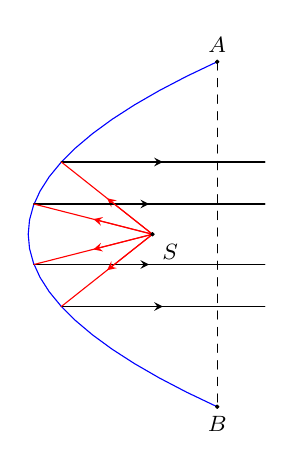
\begin{tikzpicture}[scale=0.6, font=\footnotesize, line join=round, line cap=round, >=stealth]
	\draw[domain=-3.65:3.65, blue,] plot({3/10*(\x)^2},\x);
	\coordinate (A) at (4,3.65);
	\coordinate (B) at (4,-3.65);
	\coordinate (O) at (0,0);
	\coordinate (C) at (0.12,0.64);
	\coordinate (C') at (0.12,-0.64);
	\coordinate (D) at (0.7,1.53);
	\coordinate (D') at (0.7,-1.53);
	\coordinate (F) at (5.01,1.53);
	\coordinate (F') at (5.01,-1.53);
	\coordinate (G) at (5.01,0.64);
	\coordinate (G') at (5.01,-0.64);
	\coordinate (E) at (2.63,0);
	\coordinate (H1) at (1.67,0.76);
	\coordinate (H2) at (1.67,-0.76);
	\coordinate (H3) at (1.38,0.32);
	\coordinate (H4) at (1.38,-0.32);
	\coordinate (K1) at (2.85,1.53);
	\coordinate (K2) at (2.85,-1.53);
	\coordinate (K3) at (2.56,0.64);
	\coordinate (K4) at (2.56,-0.64);
	\draw (F)--(D) (G)--(C) (F')--(D') (G')--(C') ;
	\draw[dashed] (A)--(B);
	\draw[red,->] (E)--(H1);
	\draw[->] (D)--(K1) ;
	\draw[red,->] (E)--(H3);
	\draw[->] (C)--(K3) ;
	\draw[red,->] (E)--(H4);
	\draw[->] (C')--(K4) ;
	\draw[red,->] (E)--(H2);
	\draw[->] (D')--(K2) ;
	\draw[red] (E)--(C) (E)--(D) (E)--(C') (E)--(D');
	\draw[fill=black] (A) circle (1pt) node [above] {$A$};
	\draw[fill=black] (B) circle (1pt) node [below] {$B$};
	\draw[fill=black] (E) circle (1pt) node [below right] {$S$};
	\end{tikzpicture}}
	\shortans[oly]{6,7}
\loigiai{
	Chọn hệ trục toạ độ $Oxy$ như hình vẽ bên dưới.
	\begin{center}
		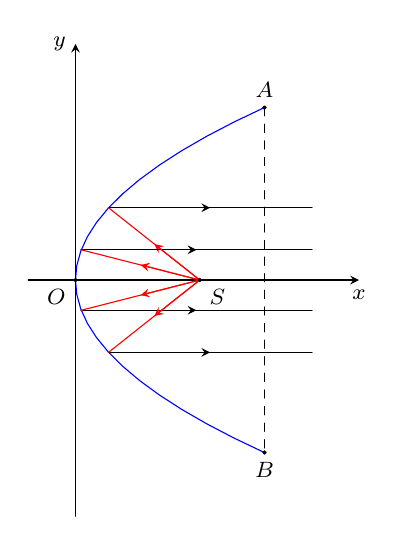
\begin{tikzpicture}[scale=0.6, font=\footnotesize, line join=round, line cap=round, >=stealth]
			\draw[domain=-3.65:3.65, blue,] plot({3/10*(\x)^2},\x);
			%\draw[gray!10] (-1,-1) grid (5,5);
			\draw[->] (-1,0)--(6,0) node[below]{$x$};
			\draw[->] (0,-5)--(0,5) node[left]{$y$};
			\coordinate (A) at (4,3.65);
			\coordinate (B) at (4,-3.65);
			\coordinate (O) at (0,0);
			\coordinate (C) at (0.12,0.64);
			\coordinate (C') at (0.12,-0.64);
			\coordinate (D) at (0.7,1.53);
			\coordinate (D') at (0.7,-1.53);
			\coordinate (F) at (5.01,1.53);
			\coordinate (F') at (5.01,-1.53);
			\coordinate (G) at (5.01,0.64);
			\coordinate (G') at (5.01,-0.64);
			\coordinate (E) at (2.63,0);
			\coordinate (H1) at (1.67,0.76);
			\coordinate (H2) at (1.67,-0.76);
			\coordinate (H3) at (1.38,0.32);
			\coordinate (H4) at (1.38,-0.32);
			\coordinate (K1) at (2.85,1.53);
			\coordinate (K2) at (2.85,-1.53);
			\coordinate (K3) at (2.56,0.64);
			\coordinate (K4) at (2.56,-0.64);
			\draw (F)--(D) (G)--(C) (F')--(D') (G')--(C') ;
			\draw[dashed] (A)--(B);
			\draw[red,->] (E)--(H1);
			\draw[->] (D)--(K1) ;
			\draw[red,->] (E)--(H3);
			\draw[->] (C)--(K3) ;
			\draw[red,->] (E)--(H4);
			\draw[->] (C')--(K4) ;
			\draw[red,->] (E)--(H2);
			\draw[->] (D')--(K2) ;
			\draw[red] (E)--(C) (E)--(D) (E)--(C') (E)--(D');
			\draw[fill=black] (A) circle (1pt) node [above] {$A$};
			\draw[fill=black] (B) circle (1pt) node [below] {$B$};
			\draw[fill=black] (E) circle (1pt) node [below right] {$S$};
			\draw[fill=black] (O) circle (1pt) node [below left] {$O$};
		\end{tikzpicture}
	\end{center}
	Gọi phương trình chính tắc của parabol có dạng $y^2=2px$, với $p>0$.\\
	Theo đề parabol đi qua điểm $A(30;20)$ nên ta có phương trình $20^2=2p\cdot 30$ suy ra $p=\dfrac{20}{3}$.\\
	Khi đó phương trình đường chuẩn của parabol đó là $x=-\dfrac{10}{3}$.\\
	Vậy khoảng cách từ bóng đèn đến đường chuẩn của parabol là $p=\dfrac{20}{3}\approx 6{,}7$ cm.
	}
\end{ex}
%Cau5
\begin{ex}%[Biên soạn tài liệu dạy học bộ KNTT-CS]%[Nguyễn Tuấn]%[0H9V5-0]
	\immini{
	Mặt cắt của một tháp làm nguội của một nhà máy là một hypebol có độ dài trục ảo bằng $80$. Khoảng cách từ nóc tháp đến tâm đối xứng bằng nửa khoảng cách từ tâm đối xứng đến đáy (hình vẽ). Tính chiều cao của tháp, biết bán kính đường tròn nóc và bán kính đường tròn đáy tháp lần lượt là $27 \sqrt{2}$ mét và $27 \sqrt{5}$ mét.
	}
	{
	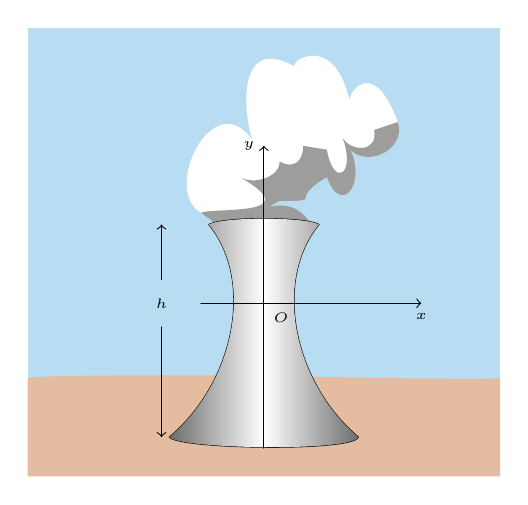
\begin{tikzpicture}[line join=round, line cap=round,scale=1,transform shape]
		\definecolor{lightcornflowerblue}{rgb}{0.6, 0.81, 0.93}
		\definecolor{tumbleweed}{rgb}{0.87, 0.67, 0.53}
		\definecolor{dimgray}{rgb}{0.41, 0.41, 0.41}
		\definecolor{battleshipgrey}{rgb}{0.52, 0.52, 0.51}
		\def\xmin{-.8} \def\xmax{2}
		\def\ymin{-1.84} \def\ymax{2}
		\fill[lightcornflowerblue!70] (-3,-2) rectangle (3,3.5);
		\tikzset{thap/.pic={
		\def\C{ %Cát
		(-3,-.65)
		..controls +(15:.2) and +(120:0) .. (0,-.62)
		..controls +(-60:0) and +(-160:0.1) .. (3,-.65)--(3,-1.9)--(-3,-1.9)--cycle
		;}
		%\draw \C;
		\fill[tumbleweed!80] \C;
		\def\D{
		(-.7,1.3)
		..controls +(-50:.9) and +(40:1.1) .. (-1.2,-1.4)
		..controls +(-50:0.2) and +(-110:0.2) .. (1.2,-1.4)
		..controls +(140:1.1) and +(-130:.9) .. (.7,1.3)
		..controls +(150:0.2) and +(30:0.2) .. (-.7,1.3)
		;}
		\draw \D;
		\fill[left color=dimgray!97,right color=dimgray!97, middle color=white] \D;
		\draw[->] (-1.3,0.6)--(-1.3,1.3);
		\draw[<-] (-1.3,-1.4)--(-1.3,0);
		}}
		\fill[white] (-.8,1.15)
		..controls +(150:.6) and +(120:1) .. (-.1,2)
		..controls +(150:.13) and +(150:1) .. (.4,3)
		..controls +(150:.13) and +(100:1) .. (1.1,2.5)
		..controls +(150:.13) and +(110:1) .. (1.7,2.3)
		..controls +(-70:.4) and +(-70:.5) .. (1,2.1)
		..controls +(-50:.6) and +(-70:.6) .. (.8,1.6)
		..controls +(-150:.6) and +(0:.6) .. (.2,1.3)
		..controls +(-150:.6) and +(120:.6) .. (.6,1)--(-.6,1)--cycle;
		\fill[battleshipgrey!80] (-.6,1)--(-.8,1.15)
		..controls +(20:.2) and +(-30:1) .. (-.3,1.6)
		..controls +(-30:.2) and +(-90:.2) .. (.2,1.8)
		..controls +(-30:.2) and +(-90:.2) .. (.5,2)--(.8,1.95)
		..controls +(-80:.5) and +(-70:.5) .. (1,2.1)
		..controls +(-60:.2) and +(-80:.3) .. (1.4,2.2)--(1.7,2.3)
		..controls +(-70:.4) and +(-70:.5) .. (1,2.1)
		..controls +(-50:.6) and +(-70:.6) .. (.8,1.6)
		..controls +(-150:.6) and +(0:.6) .. (.2,1.3)
		..controls +(-150:.6) and +(120:.6) .. (.6,1)--cycle
		;
		%%%%%%%%%%%%%%%%%%
		\path(0,-0.3)pic[scale=1]{thap};
		\draw[->] (\xmin,0)--(\xmax,0) node [below]{\tiny $x$};
		\draw[->] (0,\ymin)--(0,\ymax) node [left]{\tiny $y$};
		\node at (0,0) [below right]{\tiny $O$};
		\node at (-1.3,0) {\tiny $h$};
	\end{tikzpicture}
	}
	\shortans[oly]{120}
\loigiai{Gọi phương trình chính tắc của hypebol $(H)$ có dạng $$\dfrac{x^2}{a^2}-\dfrac{y^2}{b^2}=1\,,\heva{&a,b>0\\
	&c^2=a^2+b^2.}$$
	Theo đề
	\begin{itemize}
		\item Độ dài trục ảo $2b=80$ nên $b=40$.
		\item $(H)$ đi qua điểm $M(27\sqrt{2};y)$ ở đỉnh tháp và điểm $N(27\sqrt{5};2y)$ ở đáy tháp nên ta có hệ phương trình
		$\heva{&\dfrac{\left(27 \sqrt{2}\right)^2}{a^2}-\dfrac{y^2}{40^2}=1 \\
		&\dfrac{\left(27 \sqrt{5}\right)^2}{a^2}-\dfrac{4 y^2}{40^2}=1.}$
	\end{itemize}
	Giải hệ phương trình trên, ta được $\heva{&\dfrac{1}{a^2}=\dfrac{1}{729} \\
	&y^2=1600}$	hay $\heva{&a=27 \\&y=40.}$\\
	Do đó $h=y+2y=120$.\\
	Vậy chiều cao của tháp là $120$ mét.
	}
\end{ex}
\begin{ex}%[Biên soạn tài liệu dạy học bộ KNTT-CS]%[Nguyễn Tuấn]%[0H9V5-5]
	Hai trạm phát tín hiệu vô tuyến đặt tại hai vị trí $A$, $B$ cách nhau $200$ km. Tại cùng một thời điểm, hai trạm cùng phát tín hiệu với vận tốc $292\,000$ km/s để hai tàu thủy đang ở hai vị trí $C$, $D$ thu và đo độ lệch thời gian. Với tàu thủy tại vị trí $C$, tín hiệu từ $A$ đến sớm hơn tín hiệu từ $B$ là $0{,}0005$ s. Với tàu thủy tại vị trí $D$, tín hiệu từ $B$ đến sớm hơn tín hiệu từ $A$ là $0{,}0005$ s. Tính hiệu khoảng cách từ tàu ở vị trí $D$ đến hai trạm phát tín hiệu $A$ và $B$, từ đó tính khoảng cách từ tàu ở vị trí $D$ đến trạm tín hiệu tại $A$ biết hai tàu cách nhau $300$ km và $CD$ song song với $AB$ (làm tròn đến hàng đơn vị).
	\shortans[oly]{$279$}
\loigiai{
	\begin{center}
		\begin{tikzpicture}[scale=1, font=\footnotesize, line join=round, line cap=round, >=stealth]
			\path
			(0,0) coordinate (O)
			($(O)+(0:1.5)$) coordinate (B)
			($2*(O)-(B)$) coordinate (A)
			($(O)+(0,1.2)$) coordinate (J)
			($(J)+(0:2)$) coordinate (D)
			($2*(J)-(D)$) coordinate (C)
			;
			\draw (A)--(B) node[pos=0.6,above]{$200$};
			\draw (C)--(D) node[pos=0.6,above]{$300$};
			\draw[fill=black] (A) circle(1pt) node[above]{$A$};
			\draw[fill=black] (B) circle(1pt) node[above]{$B$};
			\draw[fill=black] (C) circle(1pt) node[above]{$C$};
			\draw[fill=black] (D) circle(1pt) node[above]{$D$};
			\draw[fill=black] (O) circle(1pt) node[below left]{$O$};
			\draw[->] (-3,0)--(3,0) node[above]{$x$};
			\draw[->] (0,-1)--(0,2) node[left]{$y$};
		\end{tikzpicture}
	\end{center}
	Với tàu thủy tại vị trí $C$, tín hiệu từ $A$ đến sớm hơn tín hiệu từ $B$ là $0{,}0005$ s nên $CA<CB$ và \[CB-CA=292\,000\cdot 0{,}0005=146\text{ km.}\]
	Tương tự với tàu thủy tại vị trí $D$, tín hiệu từ $B$ đến sớm hơn tín hiệu từ $A$ là $0{,}0005$ s nên $DA>DB$ và \[DA-DB=292\,000\cdot 0{,}0005=146\text{ km.}\]
	Do đó $C$ và $D$ đều thuộc hai nhánh của một hypebol thỏa mãn $MA-MB=146$ $\Rightarrow 2a=146 \Rightarrow a=73$ với $A$, $B$ là hai tiêu điểm.\\
	Ta có $AB=2c=200\Rightarrow c=100\Rightarrow b^2=c^2-a^2=100^2-73^2=4671$.\\
	Dựng hệ trục $Oxy$ sao cho $O$ là trung điểm $AB$, $Oy$ là trung trực của $AB$ và $B$ thuộc tia $Ox$.\\
	Suy ra $A(-100;0)$, $B(100;0)$.\\
	Phương trình chính tắc của hypebol là $\dfrac{x^2}{73^2}-\dfrac{y^2}{4671}=1$.\\
	Do $CD\parallel AB$ và tính chất đối xứng của hypebol nên $D(150;y_D)$.\\
	Vì $D$ nằm trên hypebol nên $\dfrac{150^2}{73^2}-\dfrac{y_D^2}{4671}=1\Rightarrow y_D^2=4671\left(\dfrac{150^2}{73^2}-1\right)\approx 15050{,}8$.\\
	Khi đó $DA=\sqrt{(100+150)^2+y_D^2}\approx 279$.\\
	Vậy khoảng cách từ tàu ở vị trí $D$ đến trạm tín hiệu tại $A$ khoảng $279$ km.
	}
\end{ex}
\begin{ex}%[Biên soạn tài liệu dạy học bộ KNTT-CS]%[Nguyễn Tuấn]%[0H9H5-5]
	Trong hệ tọa độ $Oxy$, điểm $M(x;y)$ có $x=\dfrac{1}{ \cos t} $; $y=\sqrt{2} \tan t$ ($0^\circ \le t \leq 180^\circ$, $ t \neq 90^\circ$). Biết điểm  $M$ luôn nằm trên một hypebol là $(H)$ khi $t$ thay đổi. Tìm tiêu cự của $(H)$. (làm tròn kết quả đến hàng phần trăm).
	\shortans[oly]{$3{,}46$}
\loigiai{
	Ta có $2x^2 - y^2 = \dfrac{2}{\cos^2 t} - 2\tan^2 t = 2$. \\
	Suy ra $(H)$ có phương trình chính tắc là $\dfrac{x^2}{1} - \dfrac{y^2}{2} =1$. \\
	Khi đó $c= \sqrt{1+2} = \sqrt{3}$. \\
	Tiêu cự của $(H)$ là $2c =2\sqrt{3} \approx 3{,}46$.
	}
\end{ex}
\begin{ex}%[Biên soạn tài liệu dạy học bộ KNTT-CS]%[Nguyễn Tuấn]%[0H9V5-9]
	Cho parabol $(P)\colon y^2=2x$. Có bao nhiêu điểm thuộc $(P)$ mà khoảng cách từ điểm đó đến tiêu điểm của $(P)$ bằng $4$?
	\shortans[oly]{2}
\loigiai{
	Parabol $(P)\colon y^2=2x$ có $p=1$ nên có tiêu điểm $F\left(\dfrac{1}{2}; 0\right)$.\\
	Gọi $M\left(x_{0}; y_{0}\right)$ là điểm cần tìm.\\
	Có $M \in (P)$ nên $y_0^2=2 x_0 \Rightarrow x_0=\dfrac{1}{2} y_0^2 \Rightarrow x_{0} \geq 0$.\\
	Khoảng cách từ $M$ đến tiêu điểm $F$ bằng $4$ nên
	$$\sqrt{\left(\dfrac{1}{2}-x_0\right)^2 + \left(0-y_0\right)^2} = 4 \Leftrightarrow x_0^2 - x_0 + \dfrac{1}{4} + y_0^2 = 16 \Leftrightarrow 4x_0^2+ 4x_0-63=0 \Leftrightarrow \hoac{& x_0=\dfrac{7}{2}\\& x_0=-\dfrac{9}{2}.}$$
	Mà $x_0 \geq 0$ nên $x_0=\dfrac{7}{2} \Rightarrow y_0^2=7 \Rightarrow y_0= \pm \sqrt{7}$.\\
	Vậy $M\left(\dfrac{7}{2}; \sqrt{7}\right)$ hoặc $M\left(\dfrac{7}{2};-\sqrt{7}\right)$.
	}
\end{ex}
\begin{ex}%[Biên soạn tài liệu dạy học bộ KNTT-CS]%[Nguyễn Tuấn]%%[0H9V5-9]
	Cho parabol $(P)\colon y^2=16x$ và đường thẳng $(d)\colon x=a$ ($a>0$). Tìm $a$ để $(d)$ cắt $(P)$ tại hai điểm phân biệt $A$ và $B$ sao cho $\widehat{AOB}=120^\circ$.
	\shortans[oly]{$5{,}33$}
\loigiai{
	\begin{center}
		\begin{tikzpicture}[scale=0.8, font=\footnotesize, line join=round, line cap=round, >=stealth]
			\def\xmin{-1}\def\xmax{3.4}\def\ymin{-3}\def\ymax{3}\pgfmathsetmacro\p{2}
			\draw[->] (\xmin-0.2,0)--(\xmax+0.2,0) node[below] {\footnotesize $x$};
			\draw[->] (0,\ymin-0.2)--(0,\ymax+0.2) node[right] {$y$};
			\clip (\xmin,\ymin) rectangle (\xmax,\ymax);
			\path
			(0,0)coordinate (O)
			(1,2) coordinate (A)
			(1,-2) coordinate (B)
			;
			\draw
			(A)--(O)--(B)
			(1,\ymin)--(1,\ymax);
			\draw[smooth,variable=\x,blue] plot ({0.25*\x*\x},{\x});
			\foreach \x/\g in {A/-30,B/30,O/-120}
			\fill (\x) circle (1.5pt) ($(\x)+(\g:5mm)$) node{$\x$};
		\end{tikzpicture}
	\end{center}
	Tọa độ giao điểm của $(d)$ và $(P)$ là $\heva{&x=a\\&y^2=16x}\Leftrightarrow\heva{&x=a\\&y^2=16a}\Leftrightarrow \heva{&x=a\\&y=\pm 4\sqrt{a}.}$\\
	Vậy giao điểm của của $(d)$ và $(P)$ là $A\left(a;-4\sqrt{a}\right)$, $B\left(a;4\sqrt{a}\right)$.\\
	Ta có $\widehat{AOB}=120^\circ\Leftrightarrow \left(\overrightarrow{OA},\overrightarrow{OB}\right)=120^\circ\Leftrightarrow \cos\left(\overrightarrow{OA},\overrightarrow{OB}\right)=-\dfrac{1}{2}$.\\
	Hay $\dfrac{a^2-16a}{\sqrt{a^2+16a}\cdot \sqrt{a^2+16a}}=-\dfrac{1}{2}\Leftrightarrow -2(a^2-16a)=a^2+16a\Leftrightarrow a=\dfrac{16}{3}>0$.\\
	Vậy $a\approx 5{,}33$.
	}
\end{ex}
\begin{ex}%[Biên soạn tài liệu dạy học bộ KNTT-CS]%[Nguyễn Tuấn]%[0H9V5-0]
	\immini[thm]{Một cái trống trường có khoảng cách giữa hai mặt trống là $1$ m. Một mặt phẳng qua trục của trống cắt phần xung quanh của trống theo hai cung của elip $(E)$ (tham khảo hình vẽ). Biết rằng elip $(E)$ có tiêu cự là $\sqrt{3}$ m , tổng các khoảng cách từ 1 điểm bất kỳ trên elip $(E)$ tới 2 tiêu điểm của elip $(E)$ là $2$ m. Hãy tính tổng diện tích của 2 mặt trống (làm tròn kết quả đến hàng phần trăm).}{
	
\begin{tikzpicture}[scale=0.5, font=\footnotesize, line join=round, line cap=round,>=stealth]
		\begin{scope}
			\fill[orange!70!black, draw=none] (-5,-3)arc (-90:-270: 0.4 and 3)--(-5,3)--plot[domain=-5:5](\x,{-1/25*(\x)^2+4})--(5,3)arc (90:-90: 0.4 and 3)--(5,-3)--plot[domain=5:-5](\x,{1/25*(\x)^2-4})--cycle;
			\fill[orange!50!black,draw=none] (5,0) ellipse (0.4 and 3);
			\fill[orange!80!black,draw=none] (5,0) ellipse (0.3 and 2.8);
			\draw[color=orange!50!black,line width=3pt] (4.9,3) arc (90:270: 0.4 and 3);
			\draw[color=orange!50!black,line width=3pt] (4,3.3) arc (90:270: 0.4 and 3.3);
			\draw[color=orange!50!black,line width=3pt] (2.5,3.7) arc (90:270: 0.4 and 3.7);
			\draw[color=orange!50!black,line width=3pt] (-2.5,3.7) arc (90:270: 0.4 and 3.7);
			\draw[color=orange!50!black,line width=3pt] (-4,3.3) arc (90:270: 0.4 and 3.3);
			\draw[color=orange!50!black,line width=3pt] (-4.9,3) arc (90:270: 0.4 and 3);
		\end{scope}
	\end{tikzpicture}}
	\shortans[oly]{$1{,}18$}
\loigiai{
	\begin{center}
		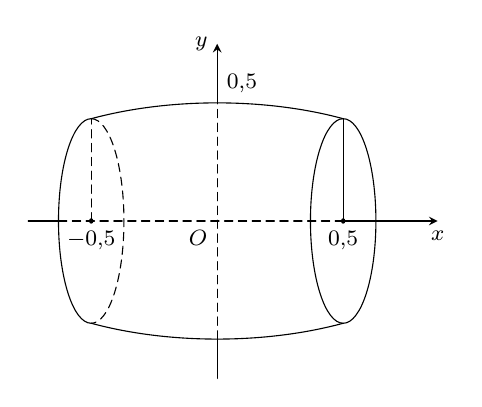
\begin{tikzpicture}[scale=1, font=\footnotesize, line join=round, line cap=round, >=stealth, yscale=0.5, xscale=0.4]
			\def\xt{-6}
			\def\xp{7}
			\def\yd{-4}
			\def\yt{4.5}
			\def\bl{8}
			\def\bn{3}
			\pgfmathsetmacro{\a}{\bl*cos(60)}
			\pgfmathsetmacro{\b}{\bn*sin(60)}
			\begin{scope}
				\draw (-\a,\b) arc (120:60:{\bl} and {\bn});
				\draw (-\a,-\b) arc (240:300: {\bl} and {\bn});
				\draw (\a,0) ellipse ({0.4*\b} and {\b});
				\draw (-\a,\b) arc (90:270:{0.4*\b} and {\b});
				\draw[densely dashed] (-\a,\b) arc (90:-90:{0.4*\b} and {\b});
			\end{scope}
			\draw[->](\a,0) node[below]{$0{,}5$} -- (\a,\b)
			(\xt,0) -- ({-\a-0.4*\b},0) ({\a},0) -- (\xp,0)node[below]{$x$} ;
			\draw[densely dashed] ({-\a-0.4*\b},0) -- (0,0)node[below left]{$O$} -- ({\a},0);
			\draw[->](0,\yd)--(0,-\bn) (0,\bn)--(0,\yt)node[left]{$y$};
			\draw[densely dashed] (0,-\bn)--(0,\bn) node[above right]{$0{,}5$}
			(-\a,0) node[below]{$-0{,}5$}--(-\a,\b);
			\fill (-\a,0) circle(2pt) (\a,0) circle(2pt);
		\end{tikzpicture}
	\end{center}
	Gọi phương trình chính tắc của elip $(E)$ là $\frac{x^{2}}{a^{2}}+\frac{y^{2}}{b^{2}}=1$.\\
	Tổng các khoảng cách từ một điểm bất kỳ trên elip đến hai tiêu điểm là $2a = 2\Rightarrow a=1$ m.\\
	Tiêu cự là $2c = \sqrt{3}\Rightarrow c=\frac{\sqrt{3}}{2}$ m.\\
	Ta có $a^{2}=b^{2}+c^{2}\Rightarrow b^{2}=a^{2}-c^{2}=1^{2}-\left(\frac{\sqrt{3}}{2}\right)^{2}=1-\frac{3}{4}=\frac{1}{4}$.
	Suy ra $b=\frac{1}{2}$ m.\\
	Phương trình của elip $(E)$ là $\dfrac{x^{2}}{1^{2}}+\dfrac{y^{2}}{\dfrac{1}{4}}=1$.\\
	Thay $x=\frac{1}{2}$ vào phương trình $(E)$ ta tính được bán kính mặt trống là $r = y = \frac{\sqrt{3}}{4}$ m.\\
	Tổng diện tích của 2 mặt trống là $S=2\cdot\pi r^{2}=2\pi\left(\frac{\sqrt{3}}{4}\right)^{2}=2\pi\cdot\frac{3}{16}=\frac{3\pi}{8} \approx 1{,}18$ m$^2$.
	}
\end{ex}
\Closesolutionfile{ans}
\indapan{4}{ans/ans-c1b1-kq}
%------------------Tự luận
\ind{PHẦN IV.} \inden{Tự luận.}
\setcounter{ex}{0}
\begin{ex}%[Biên soạn tài liệu dạy học bộ KNTT-CS]%[Nguyễn Tuấn]%[0H9H5-8]
	\immini{
	Viết phương trình chính tắc của parabol $(P)$ có tiêu điểm $F\left(\dfrac{3}{2};0\right)$.
	}{
	\begin{tikzpicture}[scale=0.6, font=\footnotesize, line join=round, line cap=round, >=stealth]
		\path
		(0,0) coordinate (O)
		(1.5,0) coordinate (F)
		;
		\draw[->] (-3,0)--(4,0) node[above]{$x$};
		\draw[->] (0,-4)--(0,4) node[right]{$y$};
		\draw[rotate=-90,smooth, samples=200, domain=-4:4] plot (\x,{(1/6)*(\x)^2});
		\draw (-1.5,4)--(-1.5,-4) node[left]{$x=-\dfrac{3}{2}$};
		\draw[fill=black] (O) circle(1pt)++(-0.2,-0.2) node{$O$};
		\draw[fill=black] (F) circle(1pt) +(0.5,0.5) node{$F\left(\dfrac{3}{2};0\right)$};
		\draw (2.5,-3) node{$y^2=6x$};
		\foreach \i in {-2,-1,...,3} \draw (\i,-0.05)--(\i,0.05);
		\foreach \j in {-3,-2,...,3} \draw (-0.05,\j)--(0.05,\j);
	\end{tikzpicture}
	}
\loigiai{
	$(P)$ có tiêu điểm $F\left(\dfrac{3}{2};0\right)$, suy ra $\dfrac{p}{2}=\dfrac{3}{2}\Rightarrow p=3$.\\
	Vậy $(P)$ có phương trình $y^2=6x$.
	}
\end{ex}
\begin{ex}%[Biên soạn tài liệu dạy học bộ KNTT-CS]%[Nguyễn Tuấn]%[0H9H5-5]
	Viết phương trình chính tắc của hypebol $ (H)$, biết $ (H)$ đi qua điểm $ M\left(3\sqrt{2};-4\right)$ và có một tiêu điểm là $F_2(5;0)$.
\loigiai{
	Phương trình chính tắc của $ (H)$ có dạng $\dfrac{x^2}{a^2}-\dfrac{y^2}{b^2}=1$, trong đó $ a,b > 0$. Do $ (H)$ có một tiêu điểm là $F_2(5;0)$ nên ta có
	$$c=5\Rightarrow a^2+b^2=c^2=25\Leftrightarrow a^2=25-b^2.$$
	Vì $ (H)$ đi qua điểm $ M(3\sqrt 2 ;4)$ nên ta có
	$$\dfrac{(3\sqrt 2)^2}{a^2}-\dfrac{4^2}{b^2}=1\Leftrightarrow \dfrac{18}{a^2}-\dfrac{16}{b^2}=1.\qquad (1)$$
	Đặt $t=b^2> 0$. Suy ra $a^2=25-t$. Thay vào $(1)$ ta được
	\begin{eqnarray*}
		& &\dfrac{18}{25-t}-\dfrac{16}{t}=1\\
		&\Leftrightarrow & 18t-16(25-t)=(25-t)t\\
		&\Leftrightarrow & t^2+9t-400=0\\
		&\Leftrightarrow &\hoac{&t=16\\&t=-25.}
	\end{eqnarray*}
	Đối chiếu với điều kiện $ t > 0$ ta được $ t=16$.\\
	Suy ra $b^2=t=16$, $a^2=25-t=9$.\\
	Vậy phương trình chính tắt của $(H)$ là $\dfrac{x^2}{9}-\dfrac{y^2}{16}=1$.}
\end{ex}
\begin{ex}%[Biên soạn tài liệu dạy học bộ KNTT-CS]%[Nguyễn Tuấn]%[0H9V5-10]
	Ăng-ten vệ tinh parabol ở hình vẽ bên có đầu thu đặt tại tiêu điểm (Hình vẽ)
	\begin{center}
		\begin{tikzpicture}
			\begin{scope}[rotate=-55]
				\fill[cyan!80!black] (0,0) -- ++(-0.5,.3)
				-- ++(0,.1) -- ++(1,0) -- ++(0,-.1)
				-- cycle;
				\fill[cyan!80!black] (0,0.2) ellipse (0.4cm and 0.1cm);
			\end{scope}
			\begin{scope}[xshift=.2cm,yshift=.2cm,rotate=-60]
				\draw[cyan!50,ultra thick,fill=cyan!80!gray] (-1.5,2.25) parabola bend (0,0) (1.5,2.25);
				\fill[cyan!20] (-1.2,2.25) parabola bend (0.1,0.2) (1.5,2.25);
				\fill[cyan!2] (1.3,2.25) parabola bend (0.4,0.3) (0.2,0.25)
				parabola [bend at start] (1.1,2.25) -- cycle;
				\draw[cyan!80!black,ultra thick] (0.05,0) -- ++(0,.5) rectangle ++(-.1,.15) coordinate (a1);
				\draw (-1.5,2.3) -- ++(0,.3) (1.5,2.3) -- ++(0,.3);
				\draw[<->] (-1.5,2.45) -- node[right,rotate=30]{240 cm}(1.5,2.45);
				\draw[dashed] (0,0) -- ++(2,0)coordinate (a2) (1.5,2.25)coordinate (b1) -- ++(0.5,0) coordinate (b2);
				\path
				(a2)++(-.1,0) coordinate (a)
				($(b1)!(a)!(b2)$) coordinate (b)
				;
				\draw[<->] (a) -- node[below,rotate=30]{160 cm}(b);
			\end{scope}
			\begin{scope}[yshift=-2.15cm]
				\foreach \i in {0.5,0.4,0.3,0.2,0.1}{
				\fill[brown!50,opacity=0.4] (-2,-\i) rectangle (5,0);
				}
				\draw[brown,line width=3pt] (-2,0) -- (5,0);
				\shade[left color=cyan!50!gray,right color=blue!70!black,middle color=white] (-0.25,0.05) rectangle (0.25,0.2);
				\fill[cyan!50!gray] (-.2,0.2) rectangle (.2,2);
				\shade[left color=cyan!50!gray,right color=blue!70!black,middle color=white] (-0.25,2) rectangle (0.25,2.15);
			\end{scope}
		\end{tikzpicture}
	\end{center}
	Giả sử đường kính miệng ăng-ten là $240$ cm, khoảng cách từ đỉnh ăng-ten tới miệng ăng-ten là $160$ cm. Tính khoảng cách từ vị trí đặt đầu thu tới đỉnh ăng-ten (đơn vị: cm).
\loigiai{
	Chọn hệ trục toạ độ sao cho gốc toạ độ trùng với đỉnh ăng-ten và trục $Ox$ đi qua đầu thu.\\
	Giả sử phương trình chính tắc của $(P)$ là $y^2=2px,(p>0)$.\\
	Nếu $x=160$ thì $y=120$ hoặc $y=-120$.\\
	Do đó, ta có $120^2=2p\cdot160\Leftrightarrow p =45$.\\
	Vậy khoảng cách từ vị trí đặt đầu thu tới đỉnh ăng-ten là $\dfrac{p}{2}=22{,}5$.
	}
\end{ex}
\begin{ex}%[Biên soạn tài liệu dạy học bộ KNTT-CS]%[Nguyễn Tuấn]%[0H9N5-2]
	Trong mặt phẳng tọa độ $Oxy$, viết phương trình chính tắc của elip $(E)$ có độ dài trục lớn là $8$, tiêu cự bằng $2\sqrt{5}$.
\loigiai{
	Gọi phương trình chính tắc của elip $(E)$ có dạng $$\dfrac{x^2}{a^2}+\dfrac{y^2}{b^2}=1\,,\heva{&a>b>0\\
	&c^2=a^2-b^2.}$$
	Theo đề
	\begin{itemize}
		\item $2a=8$, suy ra $a=4$.
		\item $2c=2\sqrt{5}$, suy ra $c=\sqrt{5}$.
	\end{itemize}
	Và $b^2=a^2-c^2=16-5=11$, suy ra $b=\sqrt{11}$.\\
	Vậy phương trình chính tắc của elip $(E)$ là $\dfrac{x^2}{16}+\dfrac{y^2}{11}=1$.
	}
\end{ex}
\begin{ex}%[Biên soạn tài liệu dạy học bộ KNTT-CS]%[Nguyễn Tuấn]%[0H9V5-0]
	Vệ tinh nhân tạo đầu tiên được Liên Xô (cũ) phóng từ Trái Đất năm $1957$. Quỹ đạo của vệ tinh đó là một đường elip nhận tâm Trái Đất là một tiêu điểm. Người ta đo được vệ tinh cách bề mặt Trái Đất gần nhất là $583$ dặm và xa nhất là $1342$ dặm ($1$ dặm xấp xỉ $1{,}609$ km). Biết bán kính Trái Đất xấp xỉ $4000$ dặm. Tính tỉ số của tiêu cự và độ dài trục lớn.
\loigiai{
	Chọn hệ trục $Oxy$ như hình sau:
	\begin{center}
		\begin{tikzpicture}[scale=1, font=\footnotesize, line join=round, line cap=round, >=stealth]
			\draw[->] (-5,0)--(5,0)node[below]{$x$};
			\draw[->] (0,-4)--(0,4)node[left]{$y$};
			\draw (0,0) ellipse (4 cm and 3 cm);
			\draw (2.6,0)  circle (1 cm);
			\coordinate (A1) at (-4,0);
			\coordinate (A2) at (4,0);
			\coordinate (B1) at (0,-3);
			\coordinate (B2) at (0,3);
			\coordinate (F1) at (-2.6,0);
			\coordinate (F2) at (2.6,0);
			\coordinate (O) at (0,0);
			\coordinate (H) at (1.6,0);
			\coordinate (K) at (3.6,0);
			\foreach \x/\y in {A1/-130,B1/-45,A2/-45,B2/45,O/-135,F1/-90,F2/-90,H/135,K/45}{\fill (\x) circle (1pt) ($(\x)+(\y:0.3cm)$) node{$\x$};}
		\end{tikzpicture}
	\end{center}
	Gọi phương trình của quỹ đạo elip có dạng $\dfrac{x^2}{a^2}+\dfrac{y^2}{b^2}=1 (a>b>0)$ và $R$ là bán kính của Trái Đất.\\
	Theo hình trên, khoảng cách từ vệ tinh đến bề mặt Trái Đất gần nhất là
	$$KA_2=F_2A_2-F_2K=(OA_2-OF_2)-F_2K=(a-c)-R.$$
	Khoảng cách từ vệ tinh đến bề mặt Trái Đất xa nhất là
	$$HA_1=OA_1+OH=OA_1+(OF_2-HF_2)=a+(c-R).$$
	Do đó, ta có hệ phương trình
	$$\heva{&a-c-R=583\\&a+c-R=1342} \Leftrightarrow \heva{&a-c=4583\\&a+c=5342} \Leftrightarrow \heva{&a=\dfrac{9925}{2}\\&c=\dfrac{759}{2}.}$$
	Vậy tỉ số của tiêu cự và độ dài trục lớn là $\dfrac{2c}{2a}=\dfrac{c}{a}=\dfrac{759}{9925}$.}
\end{ex}
\begin{ex}%[Biên soạn tài liệu dạy học bộ KNTT-CS]%[Nguyễn Tuấn]%%[0H9V5-0]
	Một cái cầu có dây cáp treo hình parabol, cầu dài $100$ m và được nâng đỡ bởi những thanh thẳng đứng treo từ cáp xuống, thanh dài nhất là $30$ m, thanh ngắn nhất là $6$ m (hình bên dưới). Tính chiều dài của thanh cách điểm giữa cầu $18$ m.
	\begin{center}
		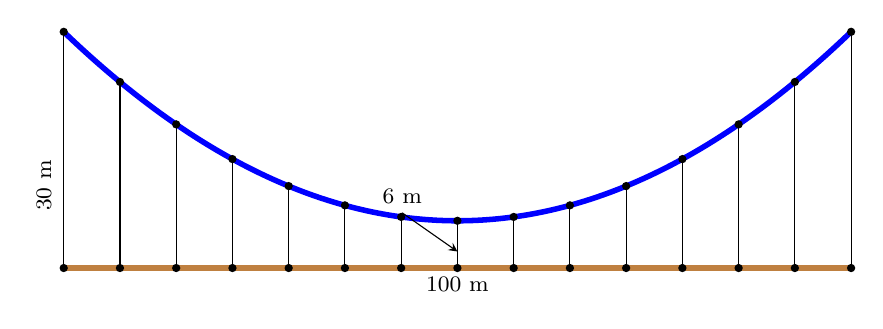
\begin{tikzpicture}[scale=0.7, font=\footnotesize, line join=round, line cap=round, >=stealth]
			\tikzset{thanh-cau/.pic={
			\pgfmathsetmacro\k{5/7};
			\draw[line width=2pt,blue,smooth,samples=100, domain=-5:5] plot (\x,{(12/125)*(\x)^2+0.6});
			\foreach \i in {-7,-6,...,7} \draw ({(\k)*(\i)},0)--({(\k)*(\i)},{(12/125)*((\k)*(\i))^2+0.6});
			\draw[line width=2pt,brown] (-5,0)--(5,0);
			\foreach \i in {-7,-6,...,7} \fill[black] ({(\k)*(\i)},0) circle (1.5pt);
			\foreach \i in {-7,-6,...,7} \fill[black] ({(\k)*(\i)},{(12/125)*((\k)*(\i))^2+0.6}) circle (1.5pt);
			}}
			\path (0,0)pic{thanh-cau};
			\draw (-7.5,1.5) node[rotate=90]{$30$ m};
			\draw (0,-0.3) node{$100$ m};
			\draw[<-] (0,0.3)--(-1,1) node[above]{$6$ m};
		\end{tikzpicture}
	\end{center}
\loigiai{
	\immini{
	Chọn hệ trục tọa độ $Oxy$ như hình vẽ bên dưới.\\
	Gọi phương trình chính tắc của parabol $(P)$ có dạng $y^2=2px$, với $p>0$.\\
	Theo đề parabol $(P)$ đi qua điểm $M(24;50)$ nên $50^2=2p\cdot 24$ hay $p=\dfrac{625}{12}$.\\
	Khi đó $(P)\colon y^2=\dfrac{625}{6}x$.\\
	Thay tọa độ điểm $N(x_N;18)$ vào phương trình $(P)$, ta được $18^2=\dfrac{625}{6}\cdot x_N$.\\
	Suy ra $x_N=\dfrac{1\,944}{625}=3{,}1104$.\\
	Vậy chiều dài của thanh cách điểm giữa cầu $18$ m là $3{,}1104+6=9{,}1104$ (m).
	}{
	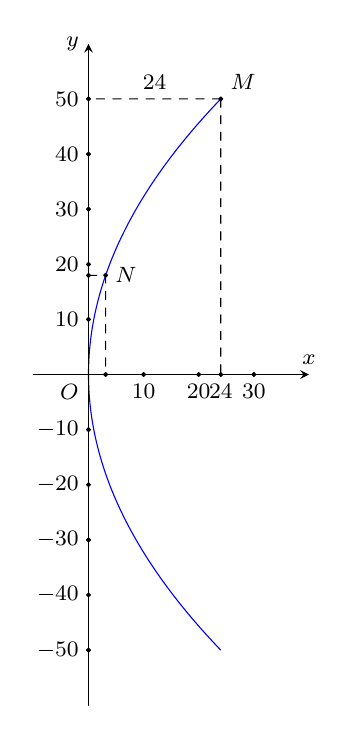
\begin{tikzpicture}[scale=0.7, font=\footnotesize, line join=round, line cap=round, >=stealth]
		\draw[rotate=-90,blue,smooth,samples=100, domain=-5:5] plot (\x,{(12/125)*(\x)^2});
		\draw[->] (-1,0)--(4,0) node[above]{$x$};
		\draw[->] (0,-6)--(0,6) node[left]{$y$};
		\draw[fill=black] (0,0) node[below left]{$O$};
		\draw [fill=black](2.4,5) coordinate(M) circle(1pt) node[above right]{$M$};
		\draw [fill=black](0.31104,1.8) coordinate(N) circle(1pt) node[right]{$N$};
		\foreach \i/\m in {1/10,2/20,3/30} \draw[fill=black] (\i,0) circle(1pt) node[below]{$\m$};
		\foreach \j/\n in {-5/-50,-4/-40,-3/-30,-2/-20,-1/-10,1/10,2/20,3/30,4/40,5/50} \draw[fill=black] (0,\j) circle(1pt) node[left]{$\n$};
		\draw[dashed] (M)--(0,5) node[above,pos=0.5]{$24$};
		\draw[dashed] (M)--(2.4,0) coordinate(M_1);
		\draw[dashed] (0,1.8) coordinate(N_2)--(N)--(0.31104,0) coordinate(N_1);
		\draw[fill=black] (M_1) circle(1pt) node[below]{$24$};
		\draw[fill=black] (N_1) circle(1pt);
		\draw[fill=black] (N_2) circle(1pt);
	\end{tikzpicture}
	}
	}
\end{ex}
%Cau7
\begin{ex}%[Biên soạn tài liệu dạy học bộ KNTT-CS]%[Nguyễn Tuấn]%[0H9H5-3]
	Trong mặt phẳng toạ độ $Oxy$, cho elip $(E)\colon 7x^2+16y^2=112$.
	\begin{enumerate}
		\item Tìm tọa độ các tiêu điểm, tọa độ các đỉnh, tiêu cự và độ dài các trục của $(E)$.
		\item Gọi $M$, $N$ là các điểm trên $(E)$ sao cho $NF_1+MF_2=7$. Tính giá trị $MF_1+NF_2$ với $F_1$, $F_2$ là hai tiêu điểm của $(E)$.
	\end{enumerate}
\loigiai{
	Ta có $(E)\colon 7x^2+16y^2=112$ hay $\dfrac{x^2}{16}+\dfrac{y^2}{7}=1$. Khi đó
	\begin{itemize}
		\item $a^2=16$, suy ra $a=4$.
		\item $b^2=7$, suy ra $b=\sqrt{7}$.
	\end{itemize}
	Và $c^2=a^2-b^2=9$, suy ra $c=3$.
	\begin{enumerate}
		\item Tọa độ các đỉnh $A_1(-4;0)$, $A_2(4;0)$, $B_1(0;-\sqrt{7})$, $B_2(0;\sqrt{7})$.\\
		Độ dài trục lớn $2a=8$, độ dài trục bé $2b=2\sqrt{7}$.\\
		Tọa độ các tiêu điểm $F_1(-3;0)$, $F_2(3;0)$.\\
		Tiêu cự $2c=6$.
		\item Ta có $M$, $N$ là các điểm trên $(E)$ nên $MF_1+MF_2=8$ và $NF_1+NF_2=8$.\\
		Suy ra $MF_1+MF_2 + NF_1+NF_2=16$.\\
		Mà $NF_1+MF_2=7$ nên $MF_1+NF_2=16-(NF_1+MF_2)=16-7=9$.
	\end{enumerate}
	}
\end{ex}
\begin{ex}%[Biên soạn tài liệu dạy học bộ KNTT-CS]%[Nguyễn Tuấn]%[0H9H5-0]
	\immini{
	Thang leo gợn sóng cho trẻ em trong công viên có hai khung thép cong hình nửa elip cao $100$ cm và khoảng cách giữa hai chân là $240$ cm.
	\begin{enumerate}
		\item Hãy chọn hệ toạ độ thích hợp và viết phương trình chính tắc của elip nói trên.
		\item Tính khoảng cách thẳng đứng từ một điểm cách chân khung $20$ cm lên đến khung thép.
	\end{enumerate}
	}{
	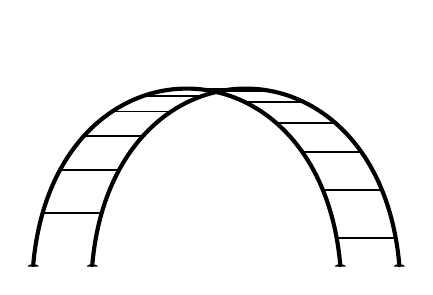
\begin{tikzpicture}[scale=3, font=\footnotesize, line join=round, line cap=round, >=stealth]
		\tikzset{
		chan/.pic={\fill[black](0,0) .. controls ++(-110:5mm) and ++(70:5mm) .. (-.7,-.5)
		-- (.7,-.5)
		.. controls ++(110:5mm) and ++(-70:5mm) .. cycle;
		}}
		\draw[black,line width=1.5pt] (0,0)pic[scale=.1,yshift=3mm]{chan} .. controls ++(85:1cm) and ++(95:1cm) .. (1.3,0)pic[scale=.1,yshift=3mm]{chan}
		\foreach \i in {8,16,24,...,96}{
		coordinate[pos=\i*0.01](A\i)
		};
		\draw[xshift=-.25cm,black,line width=1.5pt] (0,0)pic[scale=.1,yshift=3mm]{chan} .. controls ++(85:1cm) and ++(95:1cm) .. (1.3,0)pic[scale=.1,yshift=3mm]{chan};
		\foreach \i in {8,16,24,...,96}{
		\draw[black,line width=0.7] (A\i) -- ++(-.25,0);
		}
	\end{tikzpicture}
	}
\loigiai{
	\immini{		Chọn hệ trục như hình vẽ.
	\begin{enumerate}
		\item Ta có $\heva{& b=100\\& 2a=240} \Leftrightarrow \heva{& b=100\\& a=120.}$\\
		Phương trình chính tắc của elip là $\dfrac{x^2}{120^2}+\dfrac{y^2}{100^2}=1$.
		\item Thay $x=120-20=100$ vào phương trình elip ta có
		$$\dfrac{100^2}{120^2}+\dfrac{y^2}{100^2}=1 \Rightarrow y=100\cdot\sqrt{1-\dfrac{100^2}{120^2}} \Rightarrow y\approx 55\text{ (cm).}$$
	\end{enumerate}}
	{	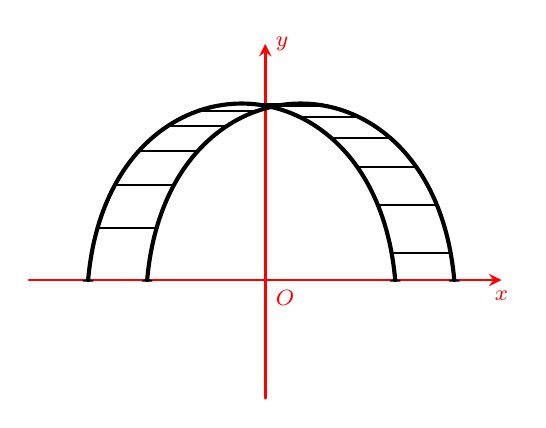
\begin{tikzpicture}[scale=3, font=\footnotesize, line join=round, line cap=round, >=stealth]
	\tikzset{
	chan/.pic={\fill[black](0,0) .. controls ++(-110:5mm) and ++(70:5mm) .. (-.7,-.5)
	-- (.7,-.5)
	.. controls ++(110:5mm) and ++(-70:5mm) .. cycle;
	}}
	\draw[->,line width = 1pt,red] (-5mm,0)--(5mm,0) node[below right]{$O$}--(15mm,0) node[below]{$x$};
	\draw[->,line width = 1pt,red] (5mm,-5mm)--(5mm,10mm) node[right]{$y$};
	\draw[black,line width=1.5pt] (0,0)pic[scale=.1,yshift=3mm]{chan} .. controls ++(85:1cm) and ++(95:1cm) .. (1.3,0)pic[scale=.1,yshift=3mm]{chan}
	\foreach \i in {8,16,24,...,96}{
	coordinate[pos=\i*0.01](A\i)
	};
	\draw[xshift=-.25cm,black,line width=1.5pt] (0,0)pic[scale=.1,yshift=3mm]{chan} .. controls ++(85:1cm) and ++(95:1cm) .. (1.3,0)pic[scale=.1,yshift=3mm]{chan};
	\foreach \i in {8,16,24,...,96}{
	\draw[black,line width=0.7] (A\i) -- ++(-.25,0);
	}
	\end{tikzpicture}}
	}
\end{ex}
\Closesolutionfile{ans}